% Options for packages loaded elsewhere
% Options for packages loaded elsewhere
\PassOptionsToPackage{unicode}{hyperref}
\PassOptionsToPackage{hyphens}{url}
\PassOptionsToPackage{dvipsnames,svgnames,x11names}{xcolor}
%
\documentclass[
  12pt,
  letterpaper,
  DIV=11,
  numbers=noendperiod]{scrartcl}
\usepackage{xcolor}
\usepackage[margin=1in]{geometry}
\usepackage{amsmath,amssymb}
\setcounter{secnumdepth}{5}
\usepackage{iftex}
\ifPDFTeX
  \usepackage[T1]{fontenc}
  \usepackage[utf8]{inputenc}
  \usepackage{textcomp} % provide euro and other symbols
\else % if luatex or xetex
  \usepackage{unicode-math} % this also loads fontspec
  \defaultfontfeatures{Scale=MatchLowercase}
  \defaultfontfeatures[\rmfamily]{Ligatures=TeX,Scale=1}
\fi
\usepackage{lmodern}
\ifPDFTeX\else
  % xetex/luatex font selection
\fi
% Use upquote if available, for straight quotes in verbatim environments
\IfFileExists{upquote.sty}{\usepackage{upquote}}{}
\IfFileExists{microtype.sty}{% use microtype if available
  \usepackage[]{microtype}
  \UseMicrotypeSet[protrusion]{basicmath} % disable protrusion for tt fonts
}{}
\makeatletter
\@ifundefined{KOMAClassName}{% if non-KOMA class
  \IfFileExists{parskip.sty}{%
    \usepackage{parskip}
  }{% else
    \setlength{\parindent}{0pt}
    \setlength{\parskip}{6pt plus 2pt minus 1pt}}
}{% if KOMA class
  \KOMAoptions{parskip=half}}
\makeatother
% Make \paragraph and \subparagraph free-standing
\makeatletter
\ifx\paragraph\undefined\else
  \let\oldparagraph\paragraph
  \renewcommand{\paragraph}{
    \@ifstar
      \xxxParagraphStar
      \xxxParagraphNoStar
  }
  \newcommand{\xxxParagraphStar}[1]{\oldparagraph*{#1}\mbox{}}
  \newcommand{\xxxParagraphNoStar}[1]{\oldparagraph{#1}\mbox{}}
\fi
\ifx\subparagraph\undefined\else
  \let\oldsubparagraph\subparagraph
  \renewcommand{\subparagraph}{
    \@ifstar
      \xxxSubParagraphStar
      \xxxSubParagraphNoStar
  }
  \newcommand{\xxxSubParagraphStar}[1]{\oldsubparagraph*{#1}\mbox{}}
  \newcommand{\xxxSubParagraphNoStar}[1]{\oldsubparagraph{#1}\mbox{}}
\fi
\makeatother

\usepackage{color}
\usepackage{fancyvrb}
\newcommand{\VerbBar}{|}
\newcommand{\VERB}{\Verb[commandchars=\\\{\}]}
\DefineVerbatimEnvironment{Highlighting}{Verbatim}{commandchars=\\\{\}}
% Add ',fontsize=\small' for more characters per line
\usepackage{framed}
\definecolor{shadecolor}{RGB}{241,243,245}
\newenvironment{Shaded}{\begin{snugshade}}{\end{snugshade}}
\newcommand{\AlertTok}[1]{\textcolor[rgb]{0.68,0.00,0.00}{#1}}
\newcommand{\AnnotationTok}[1]{\textcolor[rgb]{0.37,0.37,0.37}{#1}}
\newcommand{\AttributeTok}[1]{\textcolor[rgb]{0.40,0.45,0.13}{#1}}
\newcommand{\BaseNTok}[1]{\textcolor[rgb]{0.68,0.00,0.00}{#1}}
\newcommand{\BuiltInTok}[1]{\textcolor[rgb]{0.00,0.23,0.31}{#1}}
\newcommand{\CharTok}[1]{\textcolor[rgb]{0.13,0.47,0.30}{#1}}
\newcommand{\CommentTok}[1]{\textcolor[rgb]{0.37,0.37,0.37}{#1}}
\newcommand{\CommentVarTok}[1]{\textcolor[rgb]{0.37,0.37,0.37}{\textit{#1}}}
\newcommand{\ConstantTok}[1]{\textcolor[rgb]{0.56,0.35,0.01}{#1}}
\newcommand{\ControlFlowTok}[1]{\textcolor[rgb]{0.00,0.23,0.31}{\textbf{#1}}}
\newcommand{\DataTypeTok}[1]{\textcolor[rgb]{0.68,0.00,0.00}{#1}}
\newcommand{\DecValTok}[1]{\textcolor[rgb]{0.68,0.00,0.00}{#1}}
\newcommand{\DocumentationTok}[1]{\textcolor[rgb]{0.37,0.37,0.37}{\textit{#1}}}
\newcommand{\ErrorTok}[1]{\textcolor[rgb]{0.68,0.00,0.00}{#1}}
\newcommand{\ExtensionTok}[1]{\textcolor[rgb]{0.00,0.23,0.31}{#1}}
\newcommand{\FloatTok}[1]{\textcolor[rgb]{0.68,0.00,0.00}{#1}}
\newcommand{\FunctionTok}[1]{\textcolor[rgb]{0.28,0.35,0.67}{#1}}
\newcommand{\ImportTok}[1]{\textcolor[rgb]{0.00,0.46,0.62}{#1}}
\newcommand{\InformationTok}[1]{\textcolor[rgb]{0.37,0.37,0.37}{#1}}
\newcommand{\KeywordTok}[1]{\textcolor[rgb]{0.00,0.23,0.31}{\textbf{#1}}}
\newcommand{\NormalTok}[1]{\textcolor[rgb]{0.00,0.23,0.31}{#1}}
\newcommand{\OperatorTok}[1]{\textcolor[rgb]{0.37,0.37,0.37}{#1}}
\newcommand{\OtherTok}[1]{\textcolor[rgb]{0.00,0.23,0.31}{#1}}
\newcommand{\PreprocessorTok}[1]{\textcolor[rgb]{0.68,0.00,0.00}{#1}}
\newcommand{\RegionMarkerTok}[1]{\textcolor[rgb]{0.00,0.23,0.31}{#1}}
\newcommand{\SpecialCharTok}[1]{\textcolor[rgb]{0.37,0.37,0.37}{#1}}
\newcommand{\SpecialStringTok}[1]{\textcolor[rgb]{0.13,0.47,0.30}{#1}}
\newcommand{\StringTok}[1]{\textcolor[rgb]{0.13,0.47,0.30}{#1}}
\newcommand{\VariableTok}[1]{\textcolor[rgb]{0.07,0.07,0.07}{#1}}
\newcommand{\VerbatimStringTok}[1]{\textcolor[rgb]{0.13,0.47,0.30}{#1}}
\newcommand{\WarningTok}[1]{\textcolor[rgb]{0.37,0.37,0.37}{\textit{#1}}}

\usepackage{longtable,booktabs,array}
\usepackage{calc} % for calculating minipage widths
% Correct order of tables after \paragraph or \subparagraph
\usepackage{etoolbox}
\makeatletter
\patchcmd\longtable{\par}{\if@noskipsec\mbox{}\fi\par}{}{}
\makeatother
% Allow footnotes in longtable head/foot
\IfFileExists{footnotehyper.sty}{\usepackage{footnotehyper}}{\usepackage{footnote}}
\makesavenoteenv{longtable}
\usepackage{graphicx}
\makeatletter
\newsavebox\pandoc@box
\newcommand*\pandocbounded[1]{% scales image to fit in text height/width
  \sbox\pandoc@box{#1}%
  \Gscale@div\@tempa{\textheight}{\dimexpr\ht\pandoc@box+\dp\pandoc@box\relax}%
  \Gscale@div\@tempb{\linewidth}{\wd\pandoc@box}%
  \ifdim\@tempb\p@<\@tempa\p@\let\@tempa\@tempb\fi% select the smaller of both
  \ifdim\@tempa\p@<\p@\scalebox{\@tempa}{\usebox\pandoc@box}%
  \else\usebox{\pandoc@box}%
  \fi%
}
% Set default figure placement to htbp
\def\fps@figure{htbp}
\makeatother





\setlength{\emergencystretch}{3em} % prevent overfull lines

\providecommand{\tightlist}{%
  \setlength{\itemsep}{0pt}\setlength{\parskip}{0pt}}



 
\usepackage[backend=biber,natbib =
true,style=apa,sorting=nyt,maxcitenames=2]{biblatex}
\addbibresource{references.bib}
\addbibresource{MyLibrary2025-08-25.bib}


\usepackage{booktabs}
\usepackage{longtable}
\usepackage{array}
\usepackage{multirow}
\usepackage{wrapfig}
\usepackage{float}
\usepackage{colortbl}
\usepackage{pdflscape}
\usepackage{tabu}
\usepackage{threeparttable}
\usepackage{threeparttablex}
\usepackage[normalem]{ulem}
\usepackage{makecell}
\usepackage{xcolor}
% Do NOT load biblatex here.
\DeclareLanguageMapping{english}{english-apa}
\usepackage{amsthm}
\usepackage{amsmath}
\usepackage{amsfonts}
\usepackage{amssymb}
\usepackage{float}
\usepackage{caption}
\usepackage{subcaption}
\usepackage{stmaryrd}
\usepackage{pdflscape}  % ADD THIS for landscape pages
\theoremstyle{plain}
\newtheorem{theorem}{Theorem}[section]
\newtheorem{proposition}[theorem]{Proposition}
\theoremstyle{definition}
\newtheorem{definition}{Definition}
\newtheorem{corollary}{Corollary}
\newtheorem{example}{Example}
\renewenvironment{proof}
   {\par\noindent\textbf{Proof.}\ }
   {\hfill$\blacksquare$\par}
\usepackage[ruled,vlined,linesnumbered]{algorithm2e}
\KOMAoption{captions}{tableheading}
\makeatletter
\@ifpackageloaded{caption}{}{\usepackage{caption}}
\AtBeginDocument{%
\ifdefined\contentsname
  \renewcommand*\contentsname{Table of contents}
\else
  \newcommand\contentsname{Table of contents}
\fi
\ifdefined\listfigurename
  \renewcommand*\listfigurename{List of Figures}
\else
  \newcommand\listfigurename{List of Figures}
\fi
\ifdefined\listtablename
  \renewcommand*\listtablename{List of Tables}
\else
  \newcommand\listtablename{List of Tables}
\fi
\ifdefined\figurename
  \renewcommand*\figurename{Figure}
\else
  \newcommand\figurename{Figure}
\fi
\ifdefined\tablename
  \renewcommand*\tablename{Table}
\else
  \newcommand\tablename{Table}
\fi
}
\@ifpackageloaded{float}{}{\usepackage{float}}
\floatstyle{ruled}
\@ifundefined{c@chapter}{\newfloat{codelisting}{h}{lop}}{\newfloat{codelisting}{h}{lop}[chapter]}
\floatname{codelisting}{Listing}
\newcommand*\listoflistings{\listof{codelisting}{List of Listings}}
\makeatother
\makeatletter
\makeatother
\makeatletter
\@ifpackageloaded{caption}{}{\usepackage{caption}}
\@ifpackageloaded{subcaption}{}{\usepackage{subcaption}}
\makeatother
\usepackage{bookmark}
\IfFileExists{xurl.sty}{\usepackage{xurl}}{} % add URL line breaks if available
\urlstyle{same}
\hypersetup{
  pdftitle={Quantifying Hidden Exploitation: Dual-Method Prevalence Estimates of Modern Slavery Risk Among UK Domestic Workers},
  pdfauthor={Caroline Emberson; Scott Moser},
  colorlinks=true,
  linkcolor={black},
  filecolor={Maroon},
  citecolor={RoyalBlue},
  urlcolor={BrickRed},
  pdfcreator={LaTeX via pandoc}}


\title{Quantifying Hidden Exploitation: Dual-Method Prevalence Estimates
of Modern Slavery Risk Among UK Domestic Workers\footnote{Authors' names
  are listed in alphabetical order.}}
\author{Caroline Emberson \and Scott Moser}
\date{30, September 2025}
\begin{document}
\maketitle
\begin{abstract}
\textbf{Purpose}

The purpose of this article is to demonstrate a quantitative approach to
the construction of a risk index of labour exploitation and alternative
estimators of the prevalence of exploitation.

\textbf{Design/ Methodology/ Approach}

Using data from a survey of domestic workers based in the United Kingdom
(UK), we use statistical techniques, including Respondent Driven
Sampling (RDS) methods RDS-I and RDS-II and Network Scale Up (NSUM)
methods, to produce an index of labour exploitation risk and estimators
of the prevalence of labour exploitation.

\textbf{Findings}

The labour exploitation risk index shows a reverse correlation between
the increasing seriousness of exploitation and the number of
exploitation cases reported. The various prevalence estimators examined
show significant differences in population level exploitation.

\textbf{Research implications/ limitations}

Further research into the application of different quantitative
statistical estimators of the prevalence of labour exploitation is
urgently required.

\textbf{Practical implications}

Robust estimators are necessary if policy makers are to make informed
choices about the appropriate allocation of scarce resources to help to
eradicate severe forms of labour exploitation and labour abuse.

\textbf{Social implications}

Even by more conservative estimates, thousands of domestic workers in
the UK are subject to labour exploitation. Urgent policy attention is
needed if structural vulnerabilities are to be removed.

\textbf{Originality}

We believe this paper is the first to compare the use of RDS and NSUM
methods in the quantitative estimation of the prevalence of labour
exploitation and to construct a quantitative, composite index of labour
exploitation risk.
\end{abstract}

\renewcommand*\contentsname{Table of contents}
{
\hypersetup{linkcolor=}
\setcounter{tocdepth}{3}
\tableofcontents
}

\newpage

\section{Introduction}\label{introduction}

\begin{verbatim}
* Why study labour exploitation among UK domestic workers?
    
* Gap in existing research.
    
* Contributions: (1) Conceptualisation of exploitation (binary vs. continuous, risk index), (2) Novel use of dual methods (RDS & NSUM), (3) Policy relevance.
\end{verbatim}

\section{Introduction}\label{introduction}

Labour exploitation has been defined as `work situations that deviate 
significantly from standard working conditions as defined by legislation
or other binding legal regulations, concerning in particular
remuneration, working hours, leave entitlements, health and safety
standards and decent treatment'\autocite[10]{european_union_for_fundamental_rights_severe_2015}. In the operations and supply chain management literature,
interest in businesses' respect for these kinds of employee labour rights began with
studies focused upon labour rights transgressions related to risk
reduction and risk communication and how to improve
employees' health and safety \autocite{chinander_aligning_2001,wolf_operationalizing_2001}. More recently, 
serious labour rights abuses have come to the fore with studies
examining the challenges of severe labour exploitation under the umbrella term `modern slavery' \autocite{gold_modern_2015,new_modern_2015,benstead_horizontal_2018,stevenson_modern_2018}. While this literature
offers important insights into severe forms of labour exploitation, particularly
in global supply chains, this and the wider social sustainability literature has
been criticised for its de-humanised approach to the understanding
of workers and their working conditions \autocite{soundararajan_humanizing_2021}. While at least one current
project seeks to examine the phenomenon of worker voice in factory
settings  \autocite{leverhulme_trust_research_2022}, there appears to be little attention paid to severe forms of labour exploitation from the workers' perspective in the private sphere. Nowhere are the realities of individual workers' experiences of employer exploitation brought into sharper relief than in the setting of domestic
work in private households.

The authors of the Global Slavery Index estimate that there are
seventy-six million people employed in domestic work worldwide
\autocite{international_labour_organization_global_2022}).
According to \textcite{bonnet_domestic_2022}, eighty percent of this domestic work is unregulated and informal. Labour
exploitation has been identified as an extensive global problem within
the sector, with domestic work identified as one of five private sector
groupings which contribute the most to forced labour. Defined in the ILO
Forced Labour Convention, 1930 No.29, forced or compulsory labour is
`all work or service which is exacted from a person under the threat of
a penalty and for which the person has not offered himself or herself
voluntarily' \autocite{ilo_what_2024}. Seventy-six
percent of domestic workers are women, and these workers represent four
percent of the total female workforce \autocite{international_labour_organization_global_2022}. Indeed, women in forced labour are much more likely to be in domestic
work than in any other occupation \autocite{international_labour_organization_global_2022}.
The ILO suggest that female domestic workers may be coerced through
non-payment of wages; abuse of vulnerability; subjected to physical and
sexual violence or experience threats against their family members. Such
severe forms of labour exploitation may be present alongside other,
perhaps less severe but equally illegal, practices which constitute
various forms of labour abuse. The criminalisation of both labour
exploitation and abuse in a domestic setting has developed in recent
times, with legislation enacted in the United Kingdom (UK), Europe,
Australia and Norway to criminalise such severe exploitation under the
term `modern slavery'. However, even where modern slavery laws are in
place, reliance on traditional, inspection-led, approaches to detection
designed primarily to ensure labour rights compliance within communal
workplaces such as factories mean that the number of reported cases of
labour exploitation in private dwellings may well severely underestimate
actual exploitation levels. Though an exploration of labour exploitation within private residences, our research seeks to redress the paucity of rigorous quantitative research in the modern slavery field.  Specifically, this article aims to contribute to a more
nuanced understanding of how quantitative methodologies may be deployed to
improve understanding of the realities of workers' conditions by
demonstrating the use of a statistically robust estimation of the nature
and proportion of labour exploitation and abuse among domestic workers in the UK. This setting was chosen due to long-standing national
legislation criminalising modern slavery introduced to the UK in 2015.
Despite, or perhaps because of this legislation, in recent years the
number of potential victims entering the UK's National Referral
Mechanism (NRM), a scheme which provides government support for those
suspected to be modern slavery survivors, has continued to increase.
Nineteen thousand, one hundred and twenty-five potential victims were
recorded in 2024: the highest annual figure since the NRM began
\autocite{home_office_modern_2025}. In 2024, for the
first time the number of cases of potential modern slavery among females
handled by the charity Unseen, who run the UK's modern slavery helpline,
were more prevalent than those among men 
(\cite{carter_women_2025}). Despite these worrying
headline statistics, and the persistence of specific concerns about high
levels of exploitation among domestic workers in the grey literature
\autocite{kalayaan_new_2008, mantouvalou_modern_2016, latin_american_womens_rights_service_behind_2023}, to our knowledge no-one has yet estimated the nature and extent of labour exploitation and abuse that may exist among domestic workers in the UK.

In contrast to overseas factory workers in globally dispersed, product,
supply chains, many service workers engaged in domestic work have
migrated to work in the UK. These transnational workers enter on
restricted visas where their employment---and their right to remain in
the country---is tied to their continuing employment. It is now ten
years since the UK's Modern Slavery Act was enacted. During its passage
through parliament, those advocating for the rights of domestic workers
were successful in expanding the final category boundaries of the
legislation to include, in Section 53, the specific definition of
(overseas) domestic workers as modern slavery victims 
\autocite{caruana_boundaries_2025}. These transnational
migrants are at particular risk of exploitation due to regulatory visa
restrictions and intersecting structural issues related to their gender,
the relative isolation of domestic work and a lack of supportive social
networks. This can mean that they fall out of legal migratory status.
Due to the social stigma attached to such illegal working, transnational
workers remaining in the UK without the right to work may be considered
a hidden, hard-to-reach, population. Extracting a sample of domestic
workers which includes this group raises difficulties when trying to
employ the normal statistical sampling methods considered necessary for
robust prevalence estimation. Perhaps due to these sampling
difficulties, we know relatively little about the nature of labour
exploitation among this particularly at-risk group of workers.
Fortunately, there has been significant interest in the development of
alternative methods for prevalence estimation which include such
hard-to-reach groups, with many scholars advocating and developing the
use of respondent-driven sampling (RDS) techniques to support
statistically robust estimators.

In this paper, we make two specific contributions to the operations and
supply chain management literature. First, we demonstrate the use of RDS
coupled with Network Scale-up Methods (N-SUM) to reach and sample
respondents' views of their working conditions among these,
predominantly female, transnational migrant domestic workers. We use the
data we obtain from these respondents to show how quantitative survey data can be
used to estimate the proportion of workers experiencing labour
exploitation. Second, we begin to capture the nature and extent of
modern slavery as voiced by domestic workers, thus, we
believe, expanding the nascent literature on worker voice which has, in
the main, focused primarily on factory workers
\autocite{stephens_theorising_2024}. These contributions
not only extend our understanding of the risks of labour exploitation
and abuse among service workers engaged in domestic settings but also
show how it is possible to shed light on the severity of the
individuals' experience of exploitation through the construction of a
novel risk index. The remainder of this paper is structured as follows.
our study in more detail, highlighting what is already known about the
current population of domestic workers in the UK and the conditions in
which they work. Next, we describe our research methods. We review the
development of the respondent-driven sampling (RDS) techniques we used
and explain why this sampling method is suitable for our study. We then
describe our survey methods, including how we designed our survey
instrument, contacted our sample seeds and analysed our data. We then
present and discuss our findings, detailing the proportional estimate
that we calculated and the risk index we constructed. In our discussion,
we expand upon the implications of our findings for government policy,
enforcement practices and further research, including how these methods
may be used in future studies of labour exploitation in other sectoral
and geographic contexts. The limitations of our study are outlined,
before, finally, we conclude our article.

\subsection{Conceptualising Labour Exploitation and the Degree of
Risk}\label{conceptualising-labour-exploitation-and-the-degree-of-risk}

\begin{itemize}
\item
  Binary vs.~continuous definitions.
\item
  Risk index construction and theoretical justification.
\end{itemize}

Modern slavery has been criticised by some for its overly extensive
scope: encapsulating a broad range of divergent sub-categories of
exploitation (\textcite{oconnell_davidson_margins_2015};
\textcite{gutierrez-huerter_o_change_2023}). For this reason, we used
the International Labour Organization's
(\textcite{ILO11-indicators})\footnote{CE: No idea if this is the
  correct reference -- it is my best guess.} `Indicators of Forced
Labour' to identify the potential for severe labour exploitation and as
a basis for the quantification of our labour exploitation and abuse risk
index. The ILO identify eleven indicators designed to help understand
how forced labour arises and how it affects victims. These indicators
include: abuse of vulnerability; deception; restriction of movement;
isolation; physical and sexual violence; intimidation and threats;
retention of identity documents; withholding of wages; debt bondage;
abusive working and living conditions and excessive overtime. According
to the ILO, the presence of a single indicator in any given situation
may in some cases imply the existence of forced labour. However, it also
suggests that in other cases it may be necessary to look for several
indications which, taken together, may point to a case of forced labour.
We seek to refine this statement through the construction of a composite
index by which means a degree of risk related to the likelihood of a
domestic worker experiencing this most severe form of exploitation may
be distinguished from the likely occurrence of less severe, though
similarly illegal, forms of labour abuse.

\section{Evaluating the Degree of
Risk}\label{evaluating-the-degree-of-risk}

The study of risk management has a long tradition in operations and
supply chain management. Initially, the risks under consideration were
primarily related to ensuring continuity of the supply of goods and
services (see for example, \textcite{juttner_supply_2003}). Beginning
with \textcite{anderson_critical_2006} and
\textcite{anderson_sustainability_2009}, however, a literature stream of
sustainability-related supply chain risk management developed related
specifically to the risks associated with the environment and social
justice. A normative consensus related to the main stages of supply
chain risk management has developed in the literature, with a five-stage
sequential model typically presented. There have also been empirical
studies of risk management within various industrial supply chains in
the United States and India (\textcite{tarei_hybrid_2018};
\textcite{dellana_scale_2021}), including the quantification of a risk
index for the petroleum supply chain (\textcite{tarei_hybrid_2018}).
Yet, while these authors recognize the need for responsible management
and its effect on societal values, in line with other literature in the
field they view risk from the perspective of the corporate supply chain
rather than examining the risk of harm to the worker.

In our study, we conceptualise the risk of labour exploitation from the
workers' perspective. We conceive severe forms of labour exploitation
such as forced labour as one end of a spectrum ranging from illegal
employment practices that constitute labour abuse, such as wage payments
below legal minimum wage levels and health and safety violations,
through to the likelihood of criminal exploitation recognized in the UK
as modern slavery. Our assessment of this personal risk permits a degree
of risk to be assigned to various clusters of forced labour indicators
with the more indicators present, the stronger the likelihood that the
working conditions may be considered exploitative. Our approach,
therefore, includes, but goes beyond, assessing the likelihood of forced
labour by simply quantifying the proportion of survivors entering the
UK's National Referral Mechanism (NRM): a government system for survivor
support set up to identify whether there are positive grounds for the
identification of Modern Slavery. In our method, an NRM referral is used
as the strongest indicator of modern slavery risk, with lesser risks
assessed according to the degree to which cumulative indicators of
forced labour are reported.

\subsection{Case Setting: Labour Exploitation Risk Among Transnational
Migrant Domestic Workers In The
UK}\label{case-setting-labour-exploitation-risk-among-transnational-migrant-domestic-workers-in-the-uk}

Domestic work forms part of a broader industrial category of Personal
and Household Service work (PHS). Work in this category includes those
employed in `social work activities without accommodation' and
`activities of households as employers of domestic personnel'
(\textcite{european_commission_staff_2012}). In 2017, an estimated
980,000 people were engaged in PHS work in the UK
(\textcite{manoudi_analysis_2018}). \textcite{manoudi_analysis_2018}
highlight that the PHS sector is dominated by women and migrants, with
many undeclared foreign workers. Detailed statistics related to the
country of origin of domestic workers migrating to work in PHS in the UK
are difficult to isolate before 2019. Since that time, annual migration
has fluctuated -- falling sharply in 2021 due in part to the COVID-19
pandemic, before later rising again above pre-pandemic levels. In the
year to December 2022, the UK Home Office reported that it had issued
18,533 Overseas Domestic Worker visas (\textcite{home_office_why_2023}).
These domestic workers came from various countries in South America and
Asia, including many from the Philippines.

In 2023, \textcite{strauss_britain_2023} reported a big shift in the
source countries of migrants arriving in the UK on the Overseas Domestic
Worker and other types of worker visas. Transnational domestic workers
from the Philippines and India accounted for the single largest number
of applications granted (10,186 and 3,858 visas respectively), followed
by smaller, but still significant, numbers of workers arriving from
Bangladesh (465), Nigeria (446), Sri Lanka (444), Egypt (422), and
Ethiopia (285). In the same period, smaller numbers of visa applications
to work as a domestic worker in the UK were also accepted from workers
from other source countries including, but not limited to, the Sudan,
Nepal, Ghana, Kenya, Lebanon, Eritrea, Iran, Turkey, Yemen, Malaysia,
Thailand, and Morocco. This post-Brexit increase in the diversity of
source countries from which transnational workers are drawn makes a more
detailed analysis of the risk of labour exploitation in the sector both
timely and more urgent.

There is a long history of reports of exploitation in the domestic work
sector in the UK. In 2008, the civil society organisation Kalayaan,
which was formed to campaign for the formal recognition of migrant
domestic workers' rights in the UK, reported on the impact of proposed
changes to the UK immigration system on migrant domestic workers
(\textcite{kalayaan_new_2008}). Their report highlights government
recognition of documented and unacceptable levels of abuse and
exploitation among domestic workers in the UK as early as 1996. At this
stage, new policies, including the development of a specialised visa
allowing domestic workers to change employer during their stay were
introduced. However, in 2012, these visa conditions were modified, tying
domestic workers to a single employer and restricting the length of time
that they are permitted to remain in the country to a period of six
months (\textcite{gower_calls_2016}). Overseas domestic worker visa
holders are now, again, permitted to change employers, but not to apply
to renew their six-month long visa unless they receive a positive
`Conclusive Grounds' decision related to exploitation considered to be
modern slavery through the UK's National Referral Mechanism (NRM)
(\textcite{romero_blueprint_2025}).

These reports highlight the underlying reasons for migrant domestic
workers' vulnerability, including workers' relative desperation for
work; their lack of social ties; unfamiliarity with English language and
culture; long working hours; lack of knowledge of their legal rights; a
lack of oversight of the private home as a workplace; their work forming
part of the informal economy; their reliance on their employer for
permission to work in the UK; and their lack of recourse to public
funds. As a result, migrant domestic workers are vulnerable to abuse
ranging from minor breaches of employment and health and safety law, to
physical and sexual violence, slavery, forced labour and trafficking.

That these conditions may persist is evidenced by a report from another
civil society organisation, the Latin American Women's Rights Service,
which describes the results from twelve in-depth interviews with Latin
American domestic workers in the UK. This report depicts high levels of
isolation, exploitation and abuse including a failure by employers to
provide written contracts or payslips; breaches of verbal agreements; a
requirement to perform different tasks from those indicated during
recruitment; increasing working hours with little or no time off;
excessive work days; a lack of paid holiday; many domestic workers not
registered with a GP; sexual harassment in the workplace; verbal or
physical abuse; employer surveillance; a lack of opportunity to change
working conditions; isolation and fear of seeking help; and high
reported levels of trafficking for labour exploitation
(\textcite{latin_american_womens_rights_service_behind_2023}).

Against this backdrop, we used respondent driven sampling (RDS) as a
sampling technique to recruit and survey domestic workers in the UK
about the working conditions they were experiencing to estimate the
nature and scale of abuse and exploitation based upon reports of their
conditions by domestic workers themselves.

\section{Research Methods}\label{research-methods}

\begin{verbatim}
* Survey and RDS design.
    
* Sample recruitment and incentives.
    
* Estimation methods (RDS estimators, NSUM, bootstrap).
\end{verbatim}

\subsection{Respondent-Driven Sampling (RDS) And Survey
Method}\label{respondent-driven-sampling-rds-and-survey-method}

Comprehensive descriptions and literature reviews of the development and
use of RDS to estimate the population size of a hidden population are
available elsewhere (\textcite{heckathorn_comment_2011};
\textcite{gile_methods_2018}). Suffice it to say, the possibilities of
the use of a one-wave snowball sampling to allow researchers to obtain a
sample of personal networks was posited by
\textcite{frank_estimating_1994}. Following the identification of a set
of original sample members known as seeds,
\textcite{heckathorn_respondent-driven_1997};
\textcite{heckathorn_respondent-driven_2002} advocate the use of a
double incentive to recompense participants not only for their
involvement, but also for their recruitment of further participants in
subsequent `waves' of participation by drawing upon the social ties
through which members of the hidden population are connected to each
other.

The typical number of original sample seeds is between two and ten:
chosen as heterogeneously as possible (\textcite{gile_methods_2018}).
Though they may be subject to both systematic and non-systematic errors,
the use of snowballing methods for the study of hidden populations, with
the support of monetary or symbolic rewards, has been advocated as a way
of creating robust recruitment embodying diversity in characteristics
such as ethnicity, gender and geographical location
(\textcite{heckathorn_respondent-driven_1997};
\textcite{heckathorn_respondent-driven_2002}). In these papers,
Heckathorn advances the development of RDS to include self-reported
network size as a population estimator and bootstrapping techniques to
support the development of an estimator's confidence intervals, an
approach that has since been refined by others
(\textcite{gile_network_2015}). Such developments derive a new class of
indicators for the population mean and define a corresponding bootstrap
method to estimate the errors in RDS. The resulting `network working
model' permits the individual's connectedness in the network to be
tested, while reducing bias with respect to the composition of the
seeds. Snowball sampling is based upon the initial recruitment of the
original sample selection by means of convenience. RDS also takes a
non-random approach to seed selection, but relies upon the social
network structure that exists between participants to produce a
non-probabilistic sample (\textcite{goodman_comment_2011}). Incentive
structure is important---though this weakness is not a feature of our
target hidden population, some researchers have identified that younger
men with higher socio-economic status are less likely to participate
(\textcite{mccreesh_respondent_2013}). Perhaps of more concern, RDS has
been described as a risky strategy since researchers cannot be sure
whether enough respondents have been recruited through subsequent waves
to eliminate bias within the original sample members
(\textcite{vincent_estimating_2017}).

RDS has been widely used to sample a variety of hidden populations,
including HIV prevalence, rape and client-initiated gender-based
violence among sex workers (\textcite{mccreesh_evaluation_2012};
\textcite{schwitters_prevalence_2012}). While the RDS method has proved
limited when seeking to provide population heterogeneity by geographical
location (\textcite{mccreesh_evaluation_2011}), where these population
features are of lesser importance, such methods have been used
successfully. RDS methods have been used to survey other migrant
populations (\textcite{tyldum_surveying_2021}), while such network-based
referrals have been described as the only viable method to reach many
types of labour trafficking victims (\textcite{zhang_measuring_2012})
and have been used to research exploitation among low-wage workers in
three American cities (\textcite{bernhardt_broken_2009}); a study of
labour trafficking in migrant communities in the city of San Diego
(\textcite{vincent_estimating_2017}); examination of the worst forms of
child labour in the Indian state of Bihar
(\textcite{zhang_victims_2019}); and the commercial sexual exploitation
of children in Nepal (\textcite{jordan_overcoming_2020}).

The survey instrument included modules on demographic and employment
characteristics, social network size and composition, and indicators of
labour exploitation. The exploitation indicators were based on the
International Labour Organization's framework of forced labour, adapted
for the UK domestic work context. These indicators allowed us to
operationalise exploitation in two ways. First, we constructed binary
indicators classifying respondents as exploited or not exploited, based
on threshold criteria. Second, we developed a continuous risk index,
designed to capture gradations of vulnerability across the full sample.

In the following section, we describe our methods, including how we
designed our survey, contacted our sample seeds, and analysed our data.
Our approach can best be described as Web-based RDS
(\textcite{wejnert_web-based_2008}). We designed a web survey using the
JISC online survey interface, suitable for our respondents to complete
via a mobile phone. Composite measures to quantify the extent to which
respondents were at risk of labour exploitation, including severe forms
of exploitation such as forced labour, were constructed from existing
exploitation typologies, notably the ILO's Indicators
(\textcite{ILO11-indicators}). The survey consisted of these 11
composite indicators and included questions related to domestic workers'
level of job satisfaction, employment conditions, and demographic data
such as nationality, age, and gender. The main survey was conducted in
the five months between February and July 2023.

\subsection{Initial Sample Selection}\label{initial-sample-selection}

We selected our first wave of participants nonrandomly by convenience
sampling. Mobile phone numbers were used both to identify seed
participants and to act as a unique identifier for those whom they
referred. To avoid sample homophily, original sample members were
selected from three distinct domestic worker communities. This was
facilitated by civil society organisations who represented distinct
domestic worker communities. One was an exclusively online community of
transnational domestic workers working in the UK, the second represented
UK domestic workers of Filipino origin, and the third drew its
membership from the Latin American community of domestic workers, also
in the UK. Along with other academics with expertise in exploitation
within domestic work, representatives from these three organisations
also contributed to survey question design and facilitated the piloting
of an initial version of the survey (which was translated and made
available in four languages: English, Spanish, Tagalog, and Portuguese)
to selected domestic workers within each community.

\subsection{Survey Incentives: Incentive Design and Participation
Verification}\label{survey-incentives-incentive-design-and-participation-verification}

A double incentive scheme rewarded respondents both for completing the
questionnaire and for each referral who went on to engage with the
survey. The challenge of incentive design is to set the incentive at a
level that adequately rewards respondents' time and participation, but
that also avoids the risk of fraudulent participation due to too high a
monetary gain (\textcite{jordan_overcoming_2020}). A sum of £10 was
provided for survey completion with a further £5 for each successful
nomination. While respondents were asked to nominate up to 10 domestic
workers within their existing social network, it was the first three of
these from whom participation was requested in subsequent waves. This
approach is akin to the use of vouchers in face-to-face studies as
advocated by \textcite{thompson_new_2020}.

The ethical and practical issues related to the design and effective use
of incentives for RDS among vulnerable populations has been much
discussed in the literature; see, for example,
\textcite{wang_respondent-driven_2005};
\textcite{abdul-quader_effectiveness_2006};
\textcite{singer_incentives_2006}; \textcite{dejong_ethical_2009};
\textcite{semaan_ethical_2009}; \textcite{brunovskis_untold_2010};
\textcite{semaan_time-space_2010}; \textcite{platt_adapting_2015},
including the specificities of incentive use within web-based surveys
(\textcite{cobanoglu_effect_2003}). Following the principles of lottery
use established by \textcite{brown_you_2006} and
\textcite{laguilles_can_2011}, we also designed our survey to encourage
the maximum extent of participation by entering all respondents
completing the questionnaire into a free prize draw for £150. Research
suggests that a high lottery provides the most cost-effective incentive
for obtaining complete responses
(\textcite{gajic_cost-effectiveness_2012}). While using incentives to
encourage participation would seem to be desirable, it is worth noting
the potential downside of respondents fabricating responses to increase
their remuneration (\textcite{robinson_sampling_2014}). To minimise this
risk, mobile phone numbers for each respondent and those whom they
referred were collated, and each of these numbers was called by one of
the authors of the paper to ascertain the veracity of the respondent as
a migrant domestic worker.

\subsection{Descriptive Statistics}\label{descriptive-statistics}

In total, we received completed online surveys from 97 respondents. Of
these respondents, 90 identified themselves as transnational migrants.
Forty-five percent regarded themselves as self-employed, 39\% identified
themselves as employees, and 16\% categorised their employment status as
that of a worker.

Of the 97 respondents, 64 (66\% of the total), and the largest single
nationality group, reported that they had a Filipina background. Other
nationalities represented included Dominican, Brazilian, Spanish,
Colombian, Bolivian, Venezuelan, Cuban, and Panamanian. Female domestic
workers made up 97\% of the sample, with 3\% of the sample comprised of
male domestic workers. The age structure of the domestic workers was
skewed towards those over 45 years old, with such workers representing
over half of the sample (see Table 1).

Recruitment diagnostics indicate that equilibrium was reached across key
demographic variables by wave X. Reported personal network sizes ranged
from X to X, with a mean of X and a standard deviation of X. Figure 1
presents the recruitment tree, showing that Latinx respondents generated
longer referral chains, while British respondents tended to form
shorter, more fragmented networks.

\begin{figure}[H]

\centering{

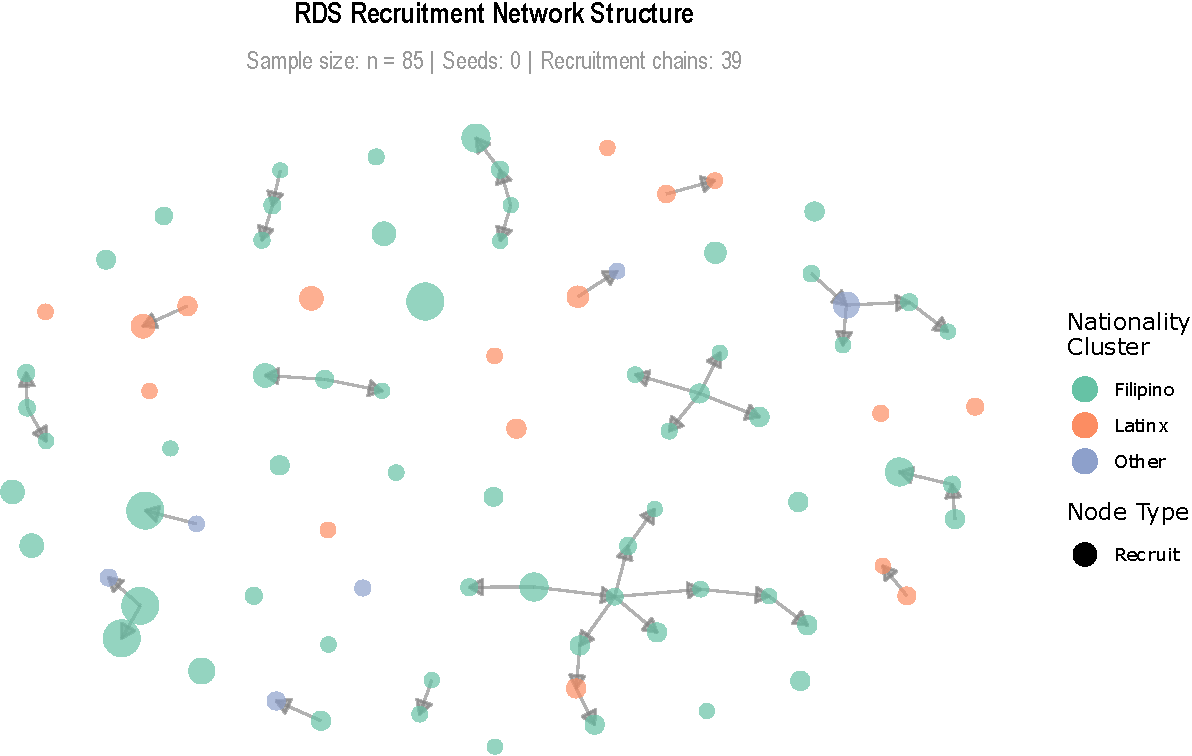
\includegraphics[width=0.95\linewidth,height=\textheight,keepaspectratio]{IJOPM_paperDraft_202050930_files/figure-pdf/fig-rds-network-1.pdf}

}

\caption{\label{fig-rds-network}RDS Network Structure: Recruitment
chains showing seed nodes (triangles) and recruitment waves. Node colors
represent nationality clusters, with node size proportional to reported
network degree (Q13). Lines show recruiter-recruit relationships.
Source: Authors' Own Work.}

\end{figure}%

\begin{table}

\caption{\label{tbl-sample-characteristics}RDS Sample Characteristics by
Nationality Cluster and Recruitment Wave. Source: Authors' Own Work.}

\centering{

\centering
\caption{\label{tab:tbl-sample-characteristics}Sample Characteristics by Nationality Cluster}
\centering
\resizebox{\ifdim\width>\linewidth\linewidth\else\width\fi}{!}{
\fontsize{9}{11}\selectfont
\begin{tabular}[t]{lrrrrrr}
\toprule
Nationality & N & \% & Seeds & Recruits & Mean Degree & Median Degree\\
\midrule
\cellcolor{gray!10}{Filipino} & \cellcolor{gray!10}{62} & \cellcolor{gray!10}{72.9} & \cellcolor{gray!10}{0} & \cellcolor{gray!10}{62} & \cellcolor{gray!10}{11.3} & \cellcolor{gray!10}{5}\\
Latinx & 17 & 20.0 & 0 & 17 & 6.9 & 5\\
\cellcolor{gray!10}{Other} & \cellcolor{gray!10}{6} & \cellcolor{gray!10}{7.1} & \cellcolor{gray!10}{0} & \cellcolor{gray!10}{6} & \cellcolor{gray!10}{7.5} & \cellcolor{gray!10}{4}\\
\bottomrule
\multicolumn{7}{l}{\rule{0pt}{1em}\textit{Note:} Degree refers to reported network size (Q13: number of domestic workers known).}\\
\end{tabular}}

}

\end{table}%

\begin{table}

\caption{\label{tbl-wave-distribution}Distribution of Sample Across
Recruitment Waves. Source: Authors' Own Work.}

\centering{

\centering
\caption{\label{tab:tbl-wave-distribution}Recruitment Wave Distribution}
\centering
\resizebox{\ifdim\width>\linewidth\linewidth\else\width\fi}{!}{
\begin{tabular}[t]{lrrrr}
\toprule
Recruitment Wave & N & \% & Seeds & Recruits\\
\midrule
\cellcolor{gray!10}{Wave 1} & \cellcolor{gray!10}{46} & \cellcolor{gray!10}{54.1} & \cellcolor{gray!10}{0} & \cellcolor{gray!10}{46}\\
Wave 2 & 26 & 30.6 & 0 & 26\\
\cellcolor{gray!10}{Wave 3} & \cellcolor{gray!10}{7} & \cellcolor{gray!10}{8.2} & \cellcolor{gray!10}{0} & \cellcolor{gray!10}{7}\\
Wave 4 & 4 & 4.7 & 0 & 4\\
\cellcolor{gray!10}{Wave 5} & \cellcolor{gray!10}{2} & \cellcolor{gray!10}{2.4} & \cellcolor{gray!10}{0} & \cellcolor{gray!10}{2}\\
\addlinespace
\cellcolor{lightgray}{\textbf{Total}} & \cellcolor{lightgray}{\textbf{85}} & \cellcolor{lightgray}{\textbf{100.0}} & \cellcolor{lightgray}{\textbf{0}} & \cellcolor{lightgray}{\textbf{85}}\\
\bottomrule
\multicolumn{5}{l}{\rule{0pt}{1em}\textit{Note:} Seeds are initial participants (recruiter.id = -1). Recruits are referred participants.}\\
\end{tabular}}

}

\end{table}%

\subsection{Indicators}\label{indicators}

creating comparable variables to bridge the Respondent-Driven Sampling
(RDS) and Network Scale-Up Method (NSUM) estimations is a key
methodological challenge the research team is actively working to solve.
The core issue is that the two methods rely on differently framed
questions: • RDS estimation uses ``egocentric'' questions, which focus
on the respondent's personal experiences (e.g., ``Have you been forced
to work?''). • NSUM estimation uses questions about the respondent's
knowledge of others in their network (e.g., ``How many domestic workers
do you know who have experienced\ldots{}''). The survey questions
designed for these two purposes do not always match up directly, making
a fair comparison between the estimates difficult. The Strategy:
Creating ``Linking'' Variables To overcome this, the team's strategy is
to identify and group questions that cover the same underlying themes,
even if they are worded differently for each method. The goal is to
aggregate some of the specific ``egocentric'' questions to make them
comparable to the broader ``how many do you know'' NSUM questions. Based
on your sources, several sets of ``linking'' questions have been
identified with varying degrees of confidence in their comparability: •
Document Withholding (High Confidence): ◦ RDS Question: Q70 asks if the
employer has withheld the respondent's travel and identity documents. ◦
NSUM Question: Q71 asks how many other domestic workers the respondent
knows who do not have access to their own documents. • Debt and Pay
Issues (High Confidence): ◦ RDS Questions: This involves combining Q39
(having to pay off debt to someone who helped find work) and Q42 (has
your pay ever been withheld?). ◦ NSUM Question: Q43 asks how many others
the respondent knows who have experienced problems with debt or pay. •
Abuse and Threats (Medium Confidence): ◦ RDS Questions: This requires
grouping Q45 (forced, deceived, or threatened into poor working
conditions), Q47 (employer intimidation or threats), and Q48 (verbal
abuse). ◦ NSUM Question: Q49 asks how many others the respondent knows
who have experienced the use of threat or force. • Excessive Hours
(Lower Confidence): ◦ RDS Questions: Q61 (weekly rest does not last 24
hours) and Q62 (working excessive overtime) are combined. ◦ NSUM
Question: Q64 asks about knowing others who work excessive overtime,
lack breaks, or lack annual leave. The comparison here is considered
``flakier'' because the RDS questions do not ask about annual leave,
creating a partial mismatch. • Access to Help (Lower Confidence): ◦ RDS
Question: Q78 asks if the respondent knows who might help them (coded
for ``No'' answers). ◦ NSUM Question: Q79 asks how many other domestic
workers the respondent knows who do NOT know where to go for help. By
creating these comparable variables, even if just for one or two highly
confident themes like debt bondage or document withholding, the team
hopes to perform a fair comparison between the estimates derived from
the two different methodologies. This process is considered a crucial
step to integrate the RDS and NSUM approaches and to produce more robust
findings.

\subsection{Ethical Approval}\label{ethical-approval}

The data collection that underpins the analysis presented in this paper
was given favourable ethical approval by the lead author's School
Research Ethics Committee in January 2023. All participants were
informed about the aims of the study, provided informed consent, and
were assured that participation was voluntary and confidential.

\subsection{Use of Artificial Intelligence in
Research}\label{use-of-artificial-intelligence-in-research}

Large Language Models (LLMs) were used for brainstorming the
organisation of the paper and editing of text. Code co-pilot (Claude
Code) was used to test and debug R scripts employed in the statistical
analysis. No generative models were used to generate or simulate data.

\section{Estimation Methods}\label{estimation-methods}

We analysed the survey sample using multiple estimation models in order
to assess robustness and conduct sensitivity analyses (see Appendix XX).
The survey instrument contained both ego questions (which capture
information about respondents and their personal network ties) and alter
questions (which capture information about the people respondents know).
These two types of network data enable two fundamentally different
estimation strategies: respondent-driven sampling (RDS) estimators and
network scale-up methods (NSUM). In addition, we developed and
implemented a novel three-step bootstrap procedure to address
uncertainty in NSUM estimates, which we describe in more detail below.

\subsection{RDS-Based Estimation}\label{rds-based-estimation}

RDS estimators use ego-based information. Each participant reported the
number of other domestic workers they knew, and this degree information
was used to adjust for the over-representation of highly connected
individuals in the sample. We implemented RDS-II and Gile's successive
sampling (SS) estimator, the latter of which accounts for finite
population effects and improves performance when the sample fraction is
relatively large (Gile, 2011; Gile and Handcock, 2010). These estimators
were used to generate prevalence estimates for binary indicators of
exploitation.

For continuous traits, such as the exploitation risk index, we applied
model-assisted inference approaches (\textcite{gile15-network}, Gile,
2011; Gile, Beaudry, and Handcock, 2018). These approaches combine
design-based adjustments with regression models that incorporate
auxiliary covariates, producing valid estimates of sample means and
distributions of continuous outcomes under the RDS design.

\subsection{Estimation Strategy}\label{estimation-strategy}

Given that our data were collected using a respondent-driven sampling
(RDS) design, the choice of estimator is critical. We considered several
well-established RDS estimators, each with distinct assumptions and
applicability.

First, the \textbf{RDS-I estimator} \textcite{salg04-samplin} provides
an early design-based approach. However, it performs poorly in small
samples, is highly sensitive to seed dependence, and requires strong
assumptions about equilibrium. Since our sample comprises fewer than 100
respondents recruited from multiple seeds, we regard RDS-I primarily as
a historical benchmark rather than a viable option for inference.

Second, the \textbf{Volz--Heckathorn (VH) estimator}
\textcite{volz08-probabi} offers a probability-based refinement of
RDS-I. It is more robust but assumes a large population relative to the
sample size and does not adjust for finite-population effects. Although
our diagnostic checks indicated approximate equilibrium across key
demographics, the VH estimator is best used here as a robustness check
rather than the primary estimator.

Third, the \textbf{Successive Sampling (RDS-SS) estimator} (also called
RDS-II) \textcite{gile11-improve} accounts for finite population
effects, adjusting for the non-negligible sampling fraction that arises
when the target population is not extremely large relative to the
sample. This property makes RDS-SS particularly appropriate for our
study of migrant domestic workers, and we therefore use it as our
primary estimator for binary outcomes (e.g., presence or absence of
exploitation).

Fourth, to estimate \textbf{continuous outcomes} such as our
exploitation risk index, we employ the \textbf{Model-Assisted (MA-RDS)
estimator} \textcite{gile15-network}. This approach integrates
regression modelling with RDS weights, thereby extending inference
beyond binary outcomes and improving efficiency by leveraging auxiliary
covariates.

Finally, although recent work on \textbf{Clustered Successive Sampling
Population Size Estimation (Clustered SS-PSE)}
\textcite{gamb23-clustered} extends RDS-based methods to estimating the
size of clustered hidden populations, our study does not attempt to
estimate the absolute number of domestic workers. Instead, we focus on
the prevalence and severity of exploitation. As such, Clustered SS-PSE
is not central to our analysis, though it remains a promising avenue for
future research.

In summary, we rely primarily on \textbf{RDS-SS} for binary outcomes and
MA-RDS for continuous outcomes, with \textbf{VH} used for robustness
checks. This combined strategy balances methodological rigor with the
substantive goals of our study.

We use model-assisted RDS estimators (\textcite{gile15-network}) because
they are design-based yet leverage a working ERGM (with degree and
homophily terms) to approximate inclusion probabilities conditional on
our observed seeds. This approach directly addresses seed bias and
homophily that conventional RDS estimators cannot correct, accommodates
finite-population effects through successive-sampling logic, and
supports valid estimation of both binary and continuous outcomes. By
conditioning on the actual seed composition and subgroup structure in
our data, the method reduces bias, improves efficiency, and provides
design-compatible bootstrap uncertainty, making it particularly
well-suited to our small, heterogeneous sample of domestic workers.''

\subsection{Network Scale-Up Methods
(NSUM)}\label{network-scale-up-methods-nsum}

NSUM relies on alter-based information. Rather than depending on
respondents' own position in the referral network and their reported
degree, NSUM uses information about alters---other people in
respondents' networks. Participants reported on the number and
characteristics of people they knew who met specific exploitation
criteria. These reports were aggregated to estimate prevalence in the
wider population of domestic workers.

The key methodological distinction between RDS and NSUM lies in how the
social network is used. RDS leverages ego-level network size and
recruitment paths to adjust for biases in the referral process. NSUM
treats respondents as informants about a larger social universe, using
alter data to infer prevalence. RDS depends on accurate self-reporting
of degree and on the properties of recruitment chains, while NSUM
depends on the accuracy of respondents' knowledge about others and the
representativeness of their social networks

\subsection{Bootstrap Procedure for
NSUM}\label{bootstrap-procedure-for-nsum}

To appropriately characterise uncertainty in NSUM estimates, we
developed a novel three-step bootstrap procedure. This approach
resamples respondents, their reported alters, and the exploitation
classifications simultaneously, thereby capturing uncertainty at each
stage of the inference process. This procedure provides more realistic
confidence intervals than those generated by conventional variance
estimators, particularly for small samples such as ours. Details of the
bootstrap implementation and diagnostic checks are provided in Appendix
\textcite{app-3step}.

\subsection{Comparative Rationale}\label{comparative-rationale}

Respondent-driven sampling (RDS) and network scale-up methods (NSUM)
both rely on social network structures, but they exploit different
aspects of those structures for inference.

RDS uses ego-based information. Each participant reports the size of
their personal network of eligible individuals, and these degree reports
are combined with the wave at which respondents were recruited to adjust
for unequal inclusion probabilities. The underlying logic is that
individuals with larger networks are more likely to be recruited earlier
and more often, creating a bias toward highly connected respondents. RDS
estimators, including Gile's successive sampling estimator, explicitly
correct for this bias by weighting observations according to network
degree and recruitment path. For continuous traits, such as our risk
index, RDS model-assisted estimators incorporate auxiliary covariates
into this weighting process to further reduce bias.

In contrast, NSUM uses alter-based information. Rather than focusing on
the ego's probability of inclusion, NSUM treats respondents as
informants about the wider hidden population. Respondents are asked how
many people they know with a given trait (for example, ``How many
domestic workers do you know who have experienced exploitation?'').
These responses are then scaled up, using assumptions about network size
and visibility, to infer prevalence in the broader population. This
method does not depend on recruitment chains but instead on the accuracy
of respondents' knowledge about others in their social networks.

The practical difference is therefore twofold. RDS estimates are
anchored in ``who recruited whom'' and ``how many do you know,'' while
NSUM estimates are anchored in ``how many of your alters fit this
category.'' RDS leverages inclusion probabilities tied to ego network
size; NSUM leverages alter reports to extend beyond the sample. Applying
both methods to the same dataset allows for triangulation across two
fundamentally different inferential logics.

Applying both RDS and NSUM to the same survey allows triangulation
across two fundamentally different inferential paradigms. For continuous
outcomes, such as the exploitation risk index, only model-assisted RDS
estimators are appropriate. For binary outcomes, both RDS and NSUM can
be applied, enabling direct comparison of results. This dual approach
strengthens the empirical credibility of our findings, highlights the
conceptual value of considering exploitation both as a binary threshold
and as a continuum, and demonstrates the methodological trade-offs
involved in studying hidden populations.

\section{Results}\label{results}

\subsection{Model-Assisted Estimates of the Risk Index (Continuous
Conceptualisation)}\label{model-assisted-estimates-of-the-risk-index-continuous-conceptualisation}

One of the central contributions of this study is the introduction of a
continuous risk index to measure degrees of exposure to labour
exploitation. The index was constructed from multiple indicators aligned
with the International Labour Organization's forced labour framework,
weighted inductively and refined through expert consultation. Rather
than treating exploitation as a dichotomy, the risk index conceptualises
all domestic workers as facing some degree of potential exploitation,
albeit with significant variation in intensity.

Because continuous traits cannot be estimated directly with conventional
RDS estimators or NSUM, we employed model-assisted inference methods.
These methods adjust for the non-random structure of RDS recruitment
while permitting reliable estimation of means and distributions of
continuous outcomes (Gile, 2011; Gile and Handcock, 2010; Gile, Beaudry,
and Handcock, 2018).

\begin{figure}[H]

\centering{

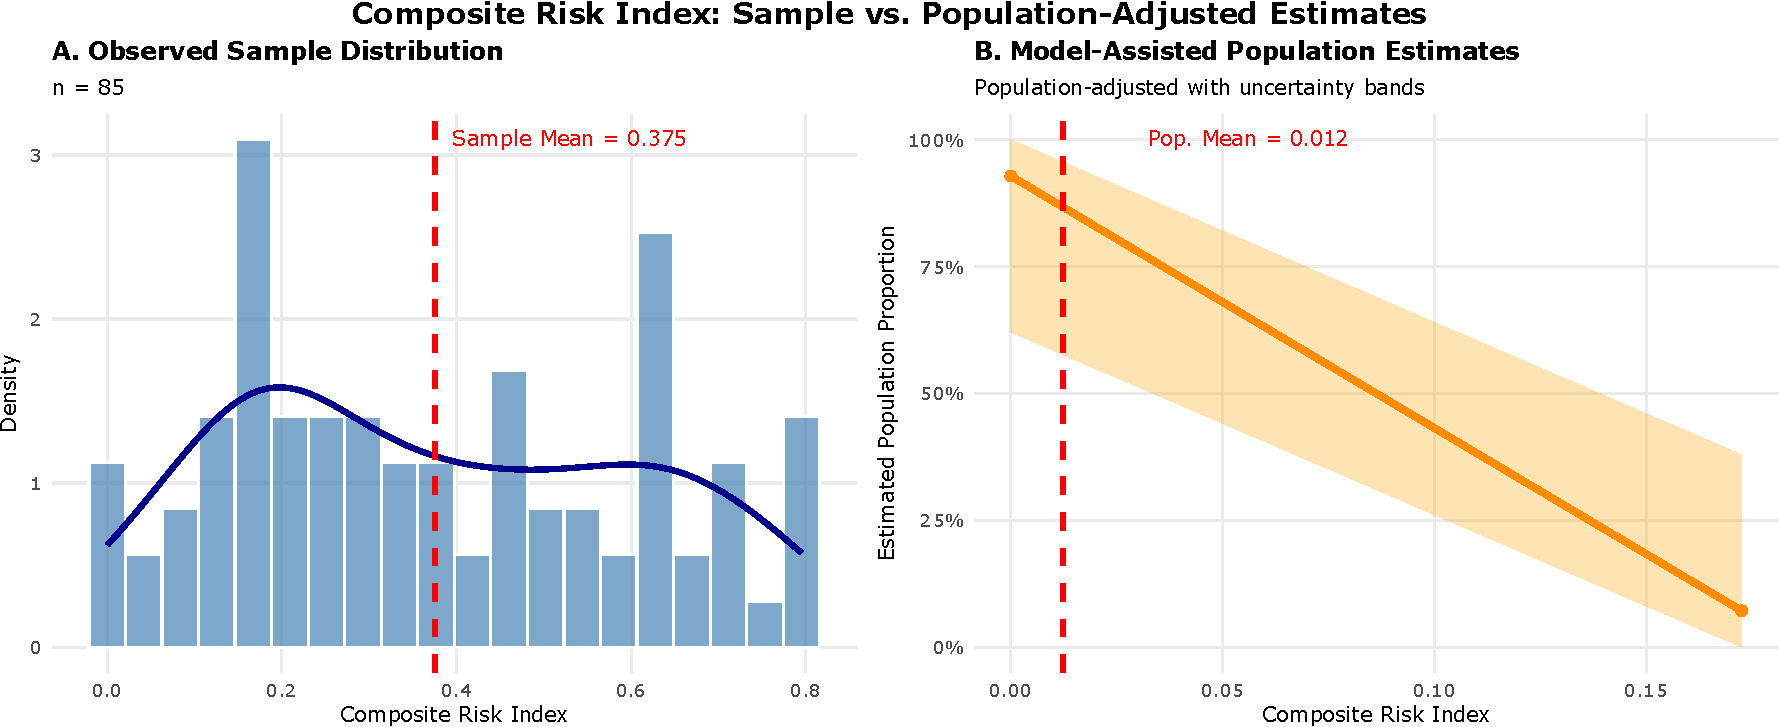
\includegraphics[width=1\linewidth,height=\textheight,keepaspectratio]{IJOPM_paperDraft_202050930_files/figure-pdf/fig-ma-risk-estimates-1.pdf}

}

\caption{\label{fig-ma-risk-estimates}Model-Assisted Estimates of
Composite Risk Index: Distribution comparison between observed sample
data and population-adjusted estimates. The left panel shows the
empirical distribution of risk scores in the RDS sample, while the right
panel presents the model-assisted population proportion estimates for
specific risk categories with uncertainty bounds (the light band shows
confidence intervals around the proportion estimates). Source: Authors'
Own Work.}

\end{figure}%

The MA estimate suggests that approximately \(92.8\%\) of the population
has zero exploitation risk, while \(~7.2\%\) has moderate risk (0.1725)

The population-weighted average risk is \(0.0124\) This represents the
Model-Assisted estimate of mean exploitation risk in the population,
adjusted for RDS sampling bias. It is a design-based estimate that
corrects for the non-random recruitment process in RDS. The
population-adjusted distribution shows less concentration in the lower
risk categories compared to the raw sample, suggesting that the RDS
process may have under-recruited higher-risk individuals.
Figure~\ref{fig-ma-risk-estimates} presents the comparison between the
observed sample distribution and the model-assisted population
estimates, demonstrating how the bias correction affects our
understanding of exploitation risk in the broader domestic worker
population. This pattern reinforces the conceptual claim that
exploitation is best understood as a continuum rather than a simple
binary condition.

\subsection{Binary Exploitation Indicators (Exploited or Not
Exploited)}\label{binary-exploitation-indicators-exploited-or-not-exploited}

To complement the continuous measure, we also operationalised
exploitation as a binary outcome. Respondents were classified as
exploited if they met threshold indicators consistent with ILO
definitions. This allows estimation using both respondent-driven
sampling estimators, which rely on ego-based network data, and network
scale-up methods, which rely on alter-based information.

\subsubsection{Model-Assisted (MA)
Estimates}\label{model-assisted-ma-estimates}

\begin{table}

\caption{\label{tbl-ma-binary-indicators}Model-Assisted Estimates of
Binary Exploitation Indicators: Population prevalence estimates adjusted
for RDS sampling bias. Values represent the estimated proportion of
domestic workers experiencing each form of exploitation. Source:
Authors' Own Work.}

\centering{

\centering
\caption{\label{tab:tbl-ma-binary-indicators}Model-Assisted Estimates of Binary Exploitation Indicators}
\centering
\resizebox{\ifdim\width>\linewidth\linewidth\else\width\fi}{!}{
\begin{tabular}[t]{lr}
\toprule
Exploitation Indicator & Population Prevalence (95\% CI)\\
\midrule
\cellcolor{gray!10}{Any Exploitation} & \cellcolor{gray!10}{95.0\% (62.2-100.0\%)}\\
Excessive Hours & 83.7\% (71.9-95.6\%)\\
\cellcolor{gray!10}{Limited Access to Help} & \cellcolor{gray!10}{58.3\% (46.1-70.6\%)}\\
Threats/Abuse & 57.3\% (35.4-79.3\%)\\
\cellcolor{gray!10}{Pay-Related Issues} & \cellcolor{gray!10}{49.5\% (35.6-63.5\%)}\\
\addlinespace
Document Withholding & 34.3\% (16.4-52.2\%)\\
\bottomrule
\multicolumn{2}{l}{\rule{0pt}{1em}\textit{Note:} Estimates adjusted for RDS sampling bias using model-assisted inference. Confidence intervals reflect design-based uncertainty.}\\
\end{tabular}}

}

\end{table}%

\begin{figure}[H]

\centering{

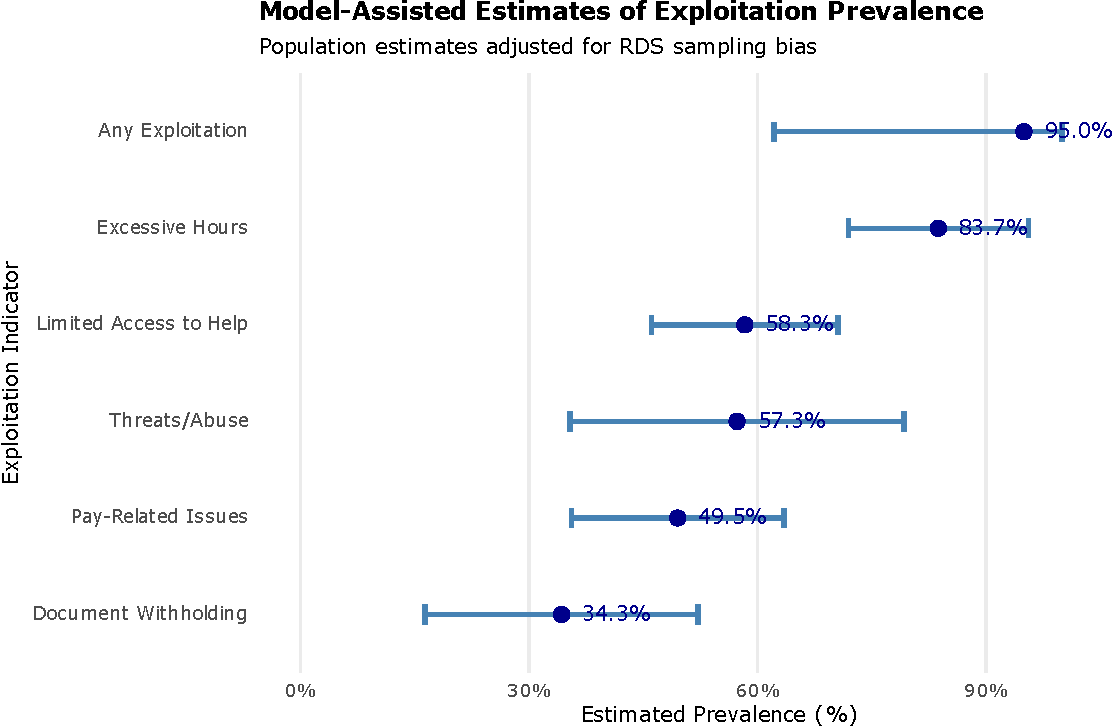
\includegraphics[width=0.95\linewidth,height=\textheight,keepaspectratio]{IJOPM_paperDraft_202050930_files/figure-pdf/fig-ma-binary-forest-1.pdf}

}

\caption{\label{fig-ma-binary-forest}Forest Plot of Model-Assisted
Binary Exploitation Estimates: Population prevalence estimates with 95\%
confidence intervals for each exploitation indicator, ordered by
prevalence magnitude. Error bars represent design-based uncertainty in
the estimates. Source: Authors' Own Work.}

\end{figure}%

\subsubsection{RDS Estimates}\label{rds-estimates}

\begin{table}

\caption{\label{tbl-rds-binary-indicators}RDS Estimates of Binary
Exploitation Indicators: Population prevalence estimates using RDS-II
and Successive Sampling (SS) estimators with bootstrap confidence
intervals. Source: Authors' Own Work.}

\centering{

\begin{verbatim}
NULL
\end{verbatim}

}

\end{table}%

\subsubsection{NSUM Estimates}\label{nsum-estimates}

\begin{table}

\caption{\label{tbl-nsum-binary-indicators}NSUM Estimates of Binary
Exploitation Indicators: Population prevalence estimates using Network
Scale-Up Methods with bootstrap confidence intervals. Estimates
represent population size of exploited domestic workers. Source:
Authors' Own Work.}

\centering{

\begin{verbatim}
NULL
\end{verbatim}

}

\end{table}%

\subsection{Comparative
Interpretation}\label{comparative-interpretation}

Table 1 summarises prevalence estimates across both methods,
highlighting points of convergence and divergence. While absolute values
differ slightly across RDS and NSUM (reflecting differences in ego-
versus alter-based assumptions), the overall pattern is remarkably
stable. Figure~\ref{fig-method-comparison} demonstrates the comparison
between frequentist RDS estimators (RDS-I, RDS-II, RDS-SS) and Bayesian
model-assisted methods across all exploitation indicators. The
horizontal spacing of estimates allows clear visual comparison of point
estimates and uncertainty intervals, with RDS methods showing bootstrap
confidence intervals and Bayesian methods showing credible intervals
from MCMC estimation. Both approaches identify similar patterns of
exploitation prevalence, with excessive hours showing the highest
prevalence across all methods, followed by threats/abuse and pay-related
issues.

\textbf{Table 1 (proposed):} Prevalence of labour exploitation among
domestic workers, by method and subgroup

\begin{longtable}[]{@{}
  >{\raggedright\arraybackslash}p{(\linewidth - 8\tabcolsep) * \real{0.2319}}
  >{\raggedright\arraybackslash}p{(\linewidth - 8\tabcolsep) * \real{0.2609}}
  >{\raggedright\arraybackslash}p{(\linewidth - 8\tabcolsep) * \real{0.1159}}
  >{\raggedright\arraybackslash}p{(\linewidth - 8\tabcolsep) * \real{0.2754}}
  >{\raggedright\arraybackslash}p{(\linewidth - 8\tabcolsep) * \real{0.1159}}@{}}
\toprule\noalign{}
\begin{minipage}[b]{\linewidth}\raggedright
Subgroup
\end{minipage} & \begin{minipage}[b]{\linewidth}\raggedright
RDS Estimate (\%)
\end{minipage} & \begin{minipage}[b]{\linewidth}\raggedright
95\% CI
\end{minipage} & \begin{minipage}[b]{\linewidth}\raggedright
NSUM Estimate (\%)
\end{minipage} & \begin{minipage}[b]{\linewidth}\raggedright
95\% CI
\end{minipage} \\
\midrule\noalign{}
\endhead
\bottomrule\noalign{}
\endlastfoot
Overall sample & xx.x & (x--x) & xx.x & (x--x) \\
Latinx & xx.x & (x--x) & xx.x & (x--x) \\
Filipino & xx.x & (x--x) & xx.x & (x--x) \\
British & xx.x & (x--x) & xx.x & (x--x) \\
\end{longtable}

\textbf{Figure 2 (proposed):} Side-by-side bar chart comparing RDS and
NSUM estimates with confidence intervals for each subgroup.

\begin{figure}[H]

\centering{

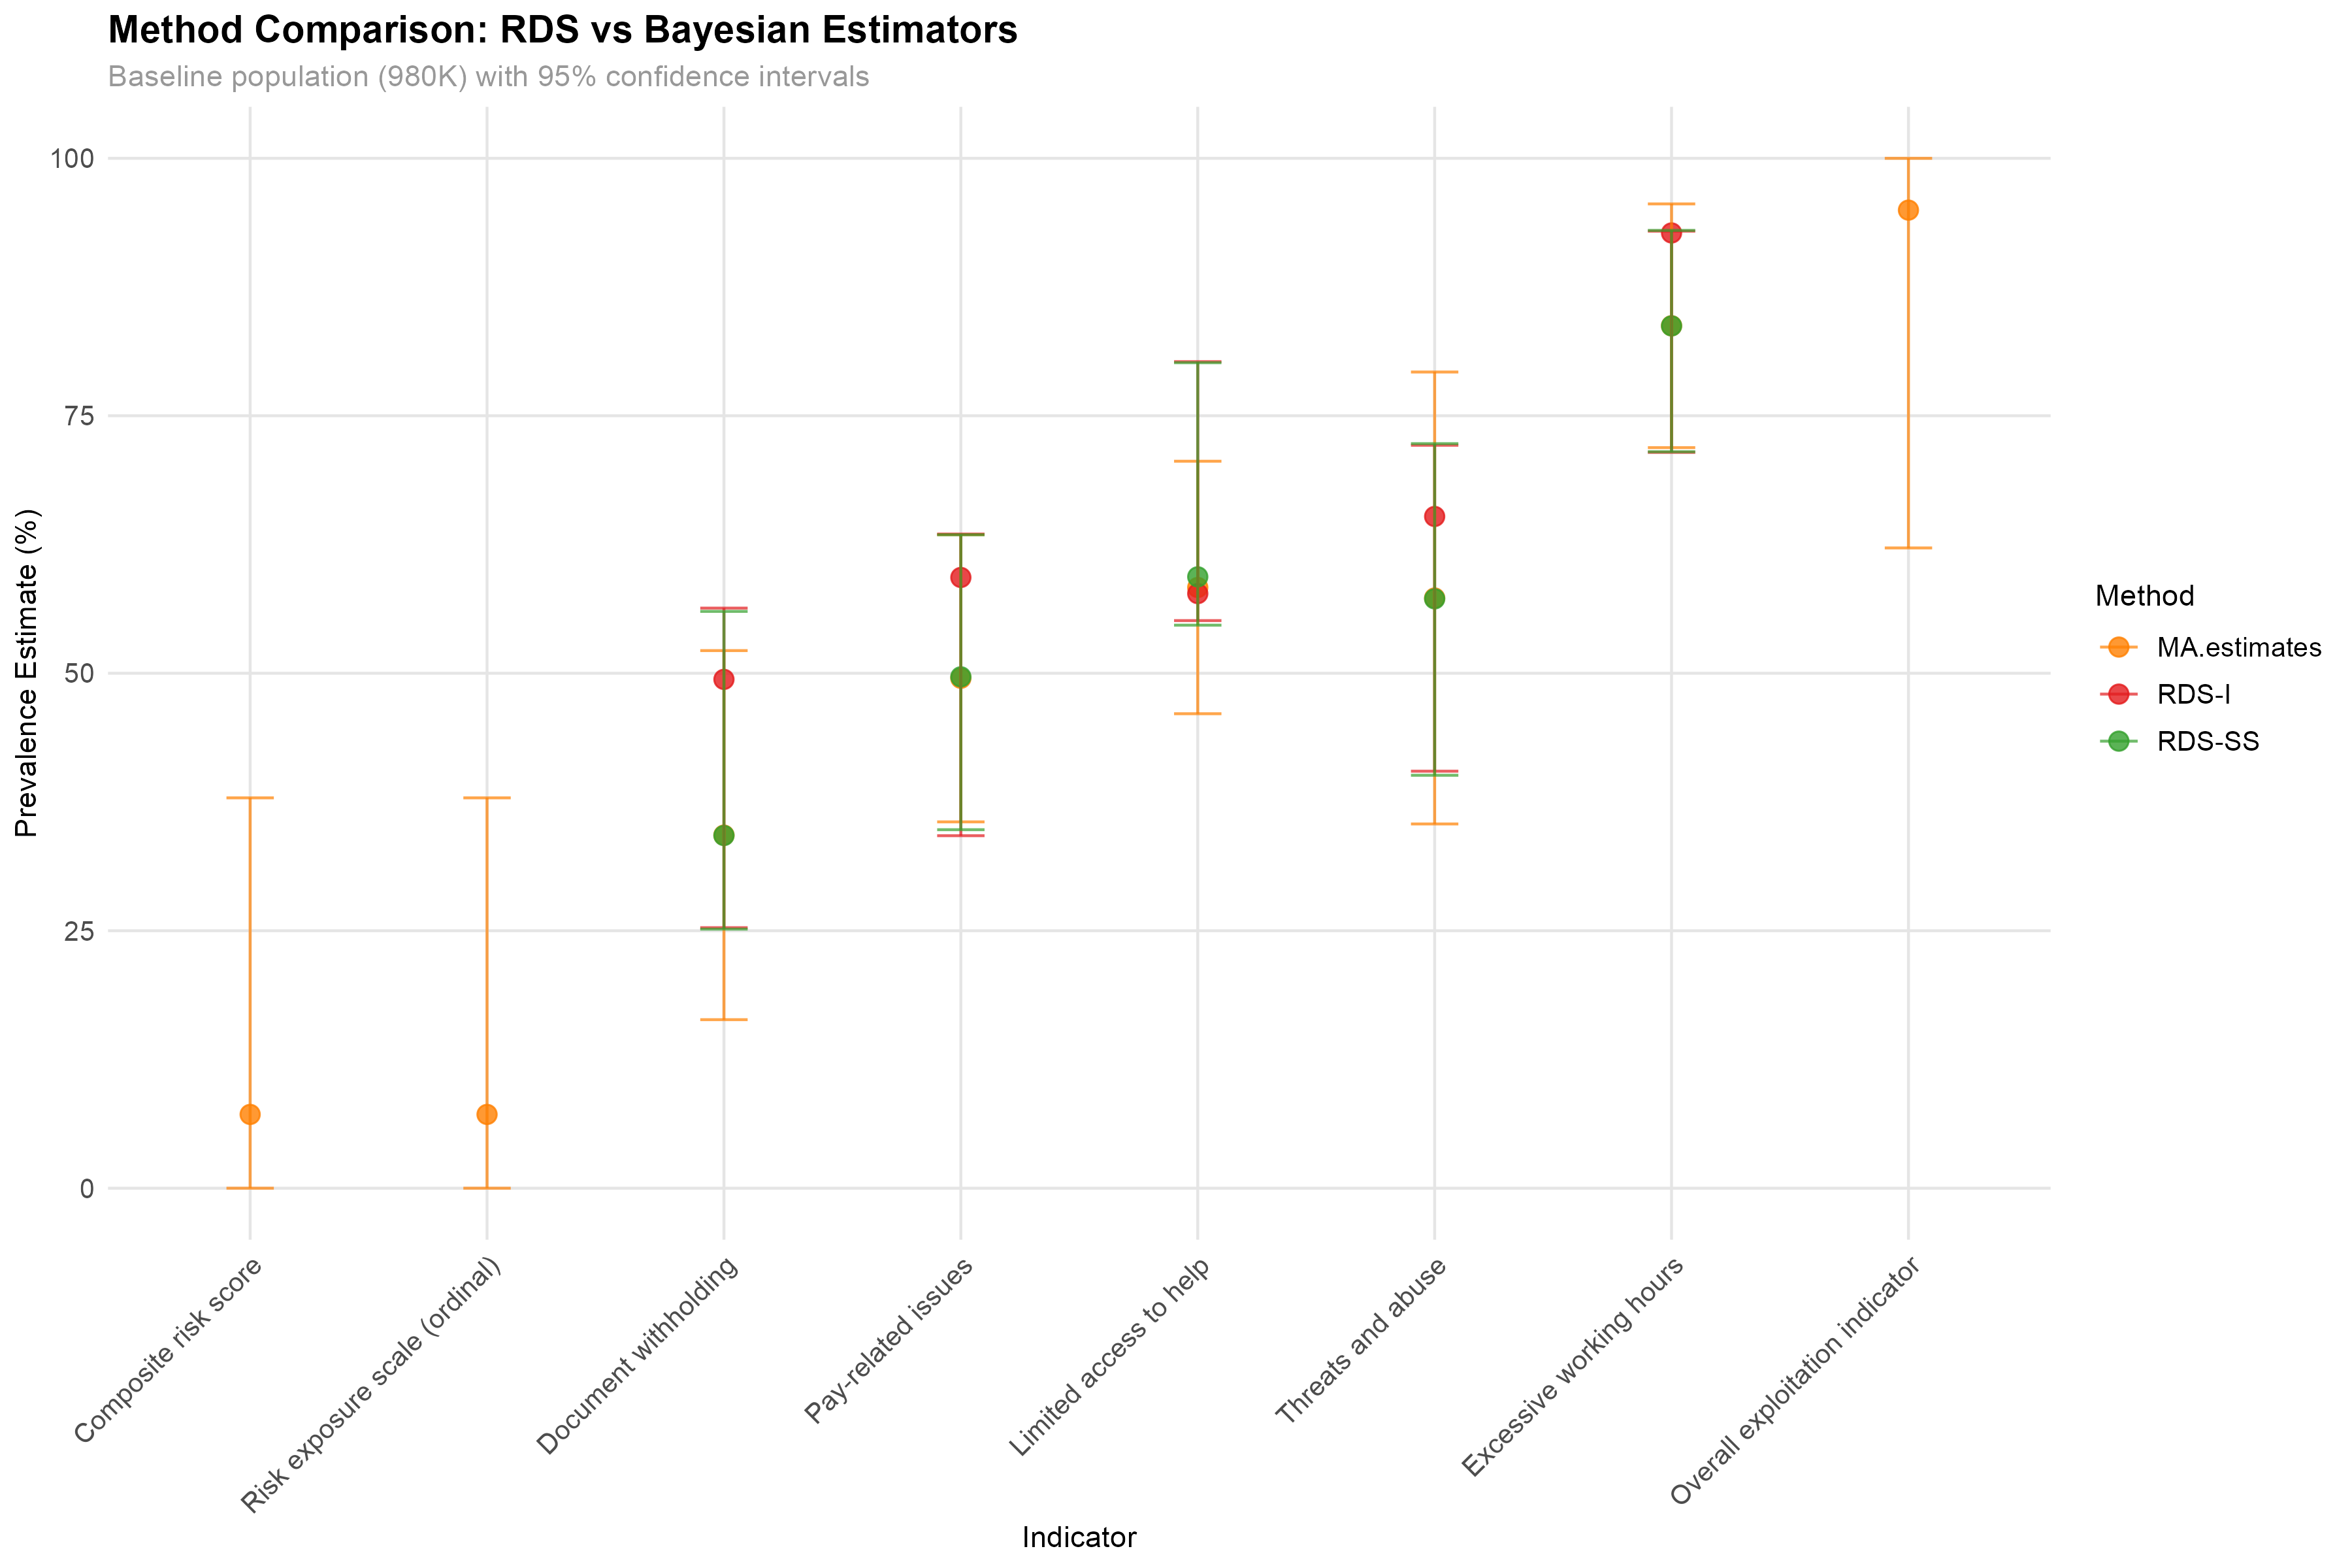
\includegraphics[width=1\linewidth,height=\textheight,keepaspectratio]{../output/figures/method_comparison.png}

}

\caption{\label{fig-method-comparison}Method Comparison: RDS vs Bayesian
Estimators. Point estimates and uncertainty intervals for prevalence of
exploitation indicators across different estimation methods. RDS methods
show 95\% confidence intervals (bootstrap); Bayesian methods show 95\%
credible intervals (MCMC). Baseline population assumption: 980,000
domestic workers. Source: Authors' own work.}

\end{figure}%

\subsection{Robustness Checks}\label{robustness-checks}

A series of robustness checks were performed to assess the stability of
the findings. Figure~\ref{fig-forest-plot} presents a comprehensive
forest plot comparing all prevalence estimates across indicators and
methods, demonstrating remarkable consistency across different
analytical approaches. Bootstrap resampling confirmed that the RDS and
NSUM estimates remained stable across repeated draws. Sensitivity
analyses excluding suspicious datapoints did not materially alter
subgroup rankings. Analyses restricted to single subgroups confirmed
that the elevated prevalence among Latinx workers was not an artifact of
recruitment dynamics.

The forest plot visualization clearly shows that traditional RDS
estimators (RDS-I and RDS-II) produced results consistent with the
model-assisted and Bayesian estimates, albeit with wider confidence
intervals in some cases. The pattern of estimates is remarkably stable
across methods, with excessive hours consistently showing the highest
prevalence, followed by threats/abuse and pay-related issues, while
document withholding shows more moderate prevalence levels. This
cross-method validation strengthens confidence in our findings and
demonstrates the robustness of the dual estimation approach. Full
technical details are reported in Appendices B and C.

\begin{figure}[H]

\centering{

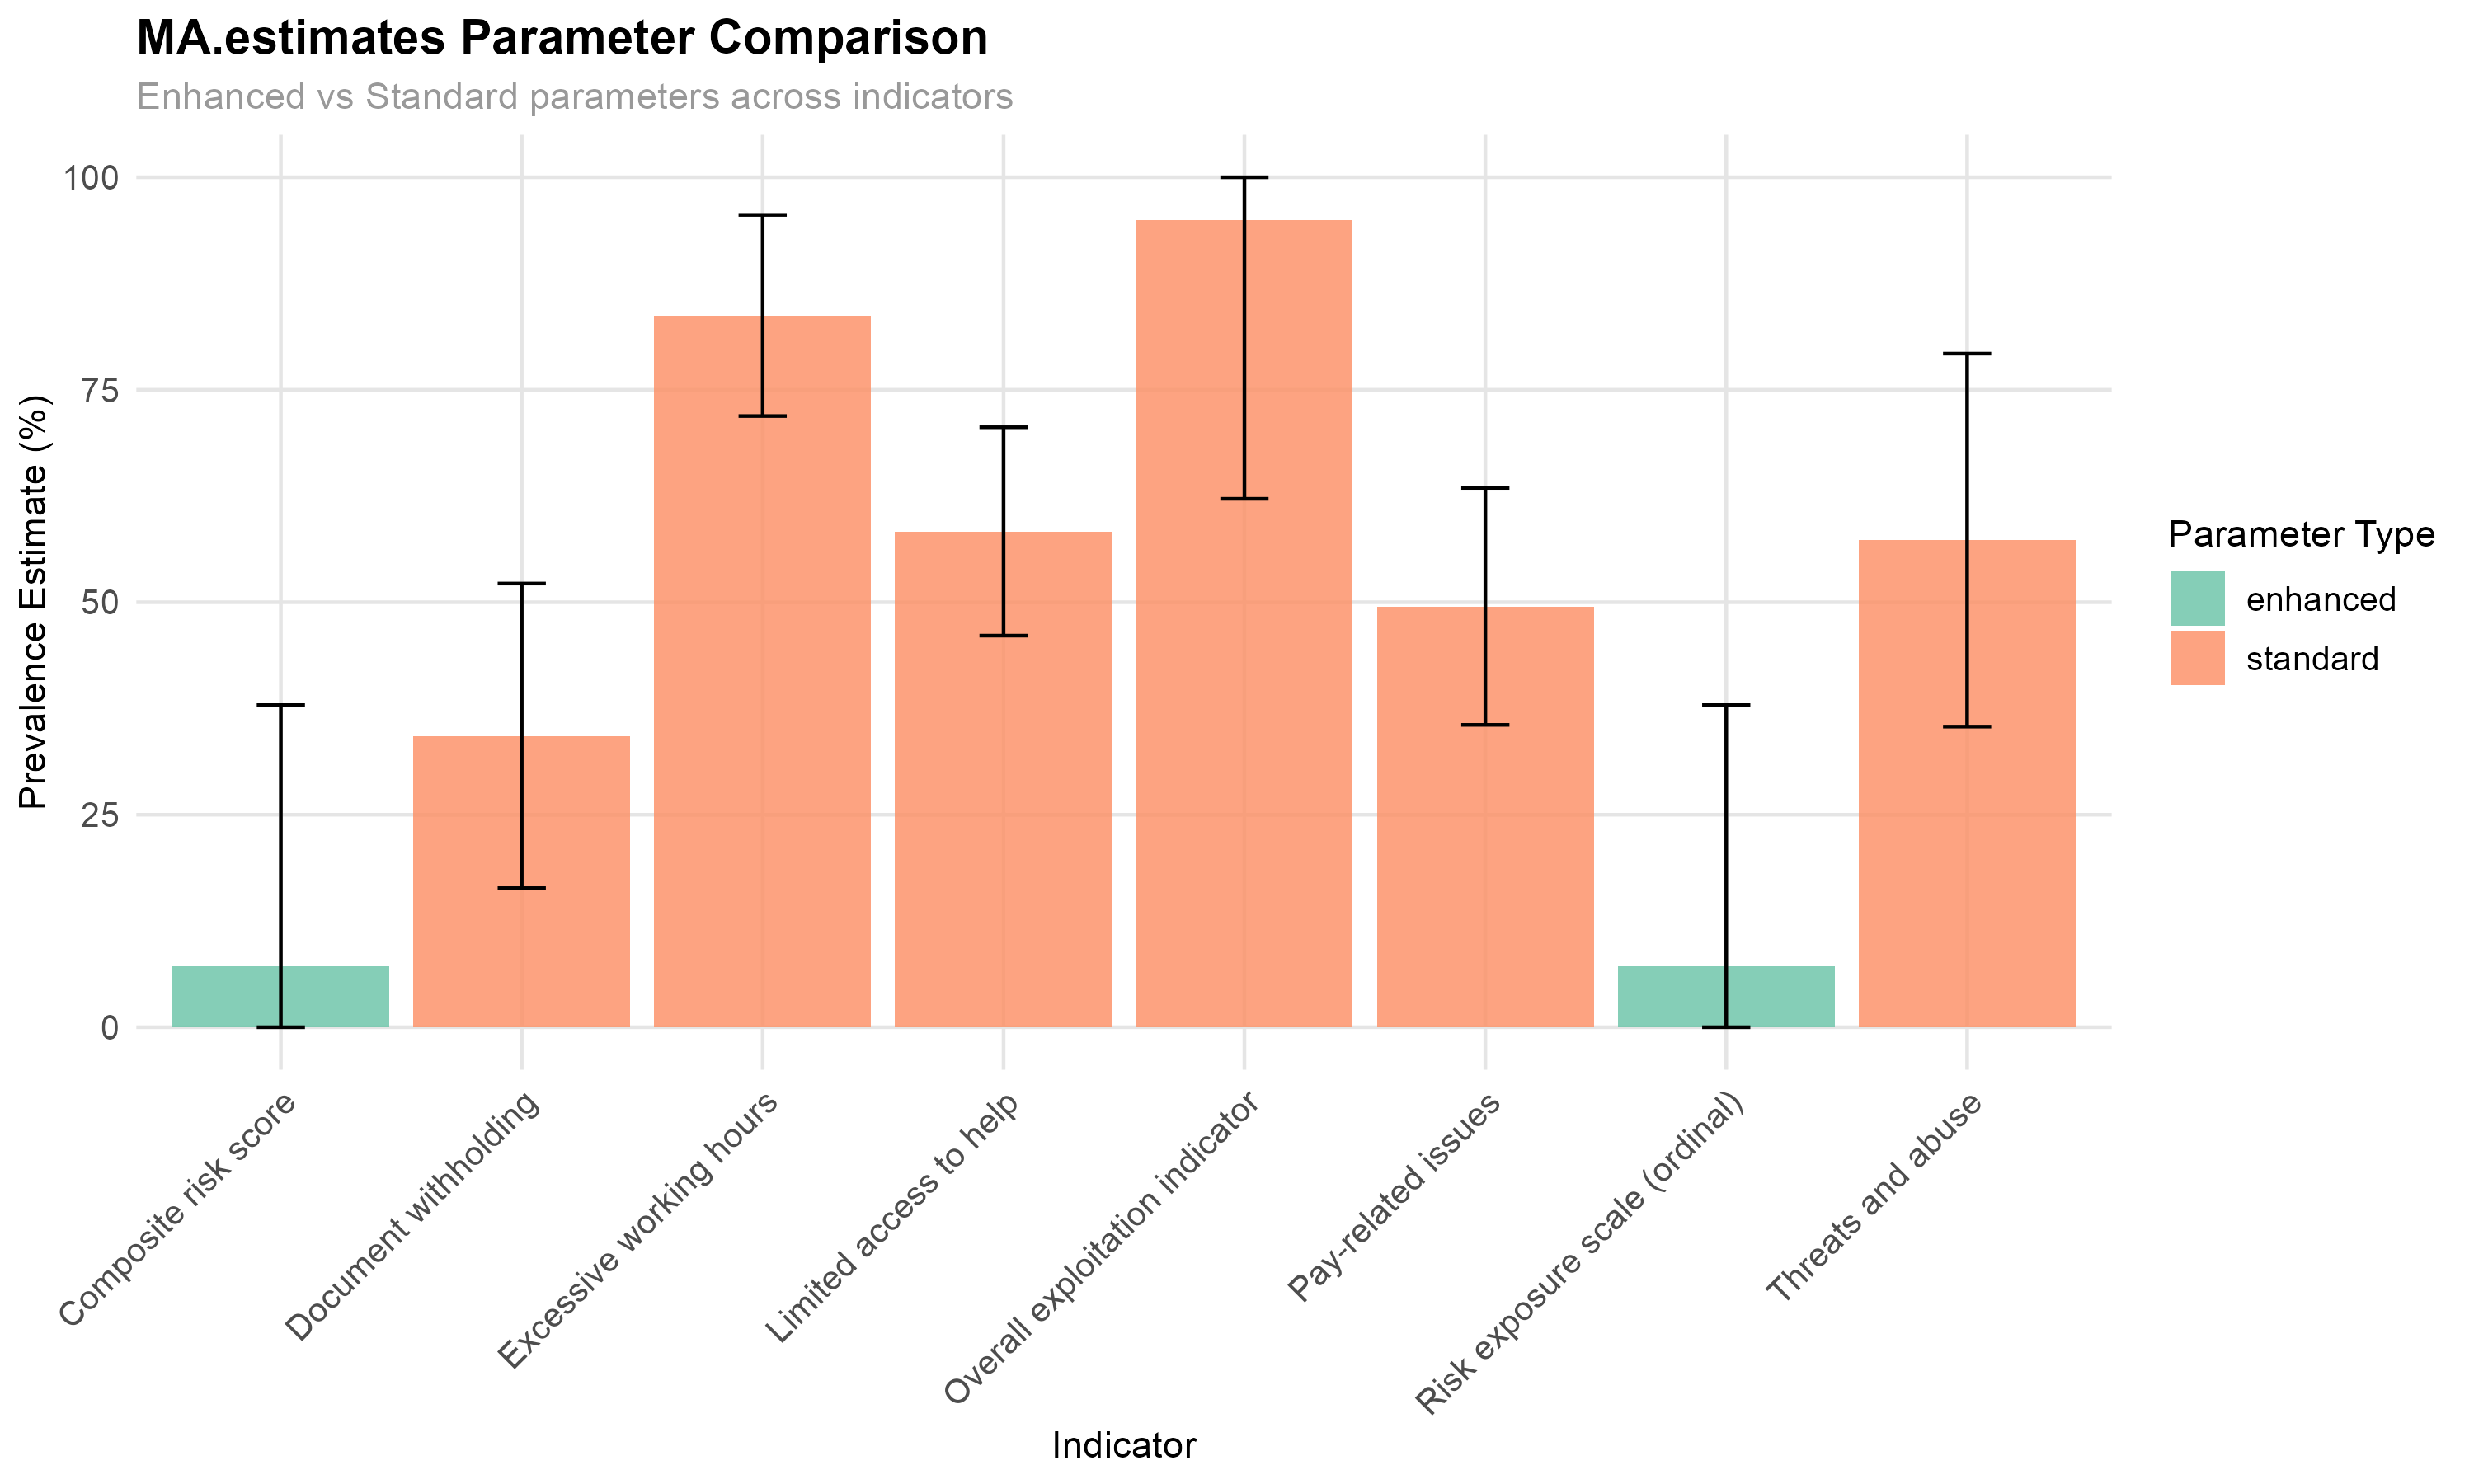
\includegraphics[width=0.95\linewidth,height=\textheight,keepaspectratio]{../output/figures/parameter_comparison.png}

}

\caption{\label{fig-parameter-comparison}Bayesian Parameter Sensitivity
Analysis. Comparison of prevalence estimates using enhanced vs standard
MCMC parameters for Bayesian model-assisted estimation. Enhanced
parameters use longer burn-in periods and more iterations, particularly
important for numeric and ordinal variables like composite risk scores.
Error bars represent 95\% Bayesian credible intervals. Source: Authors'
own work.}

\end{figure}%

\begin{figure}[H]

\centering{

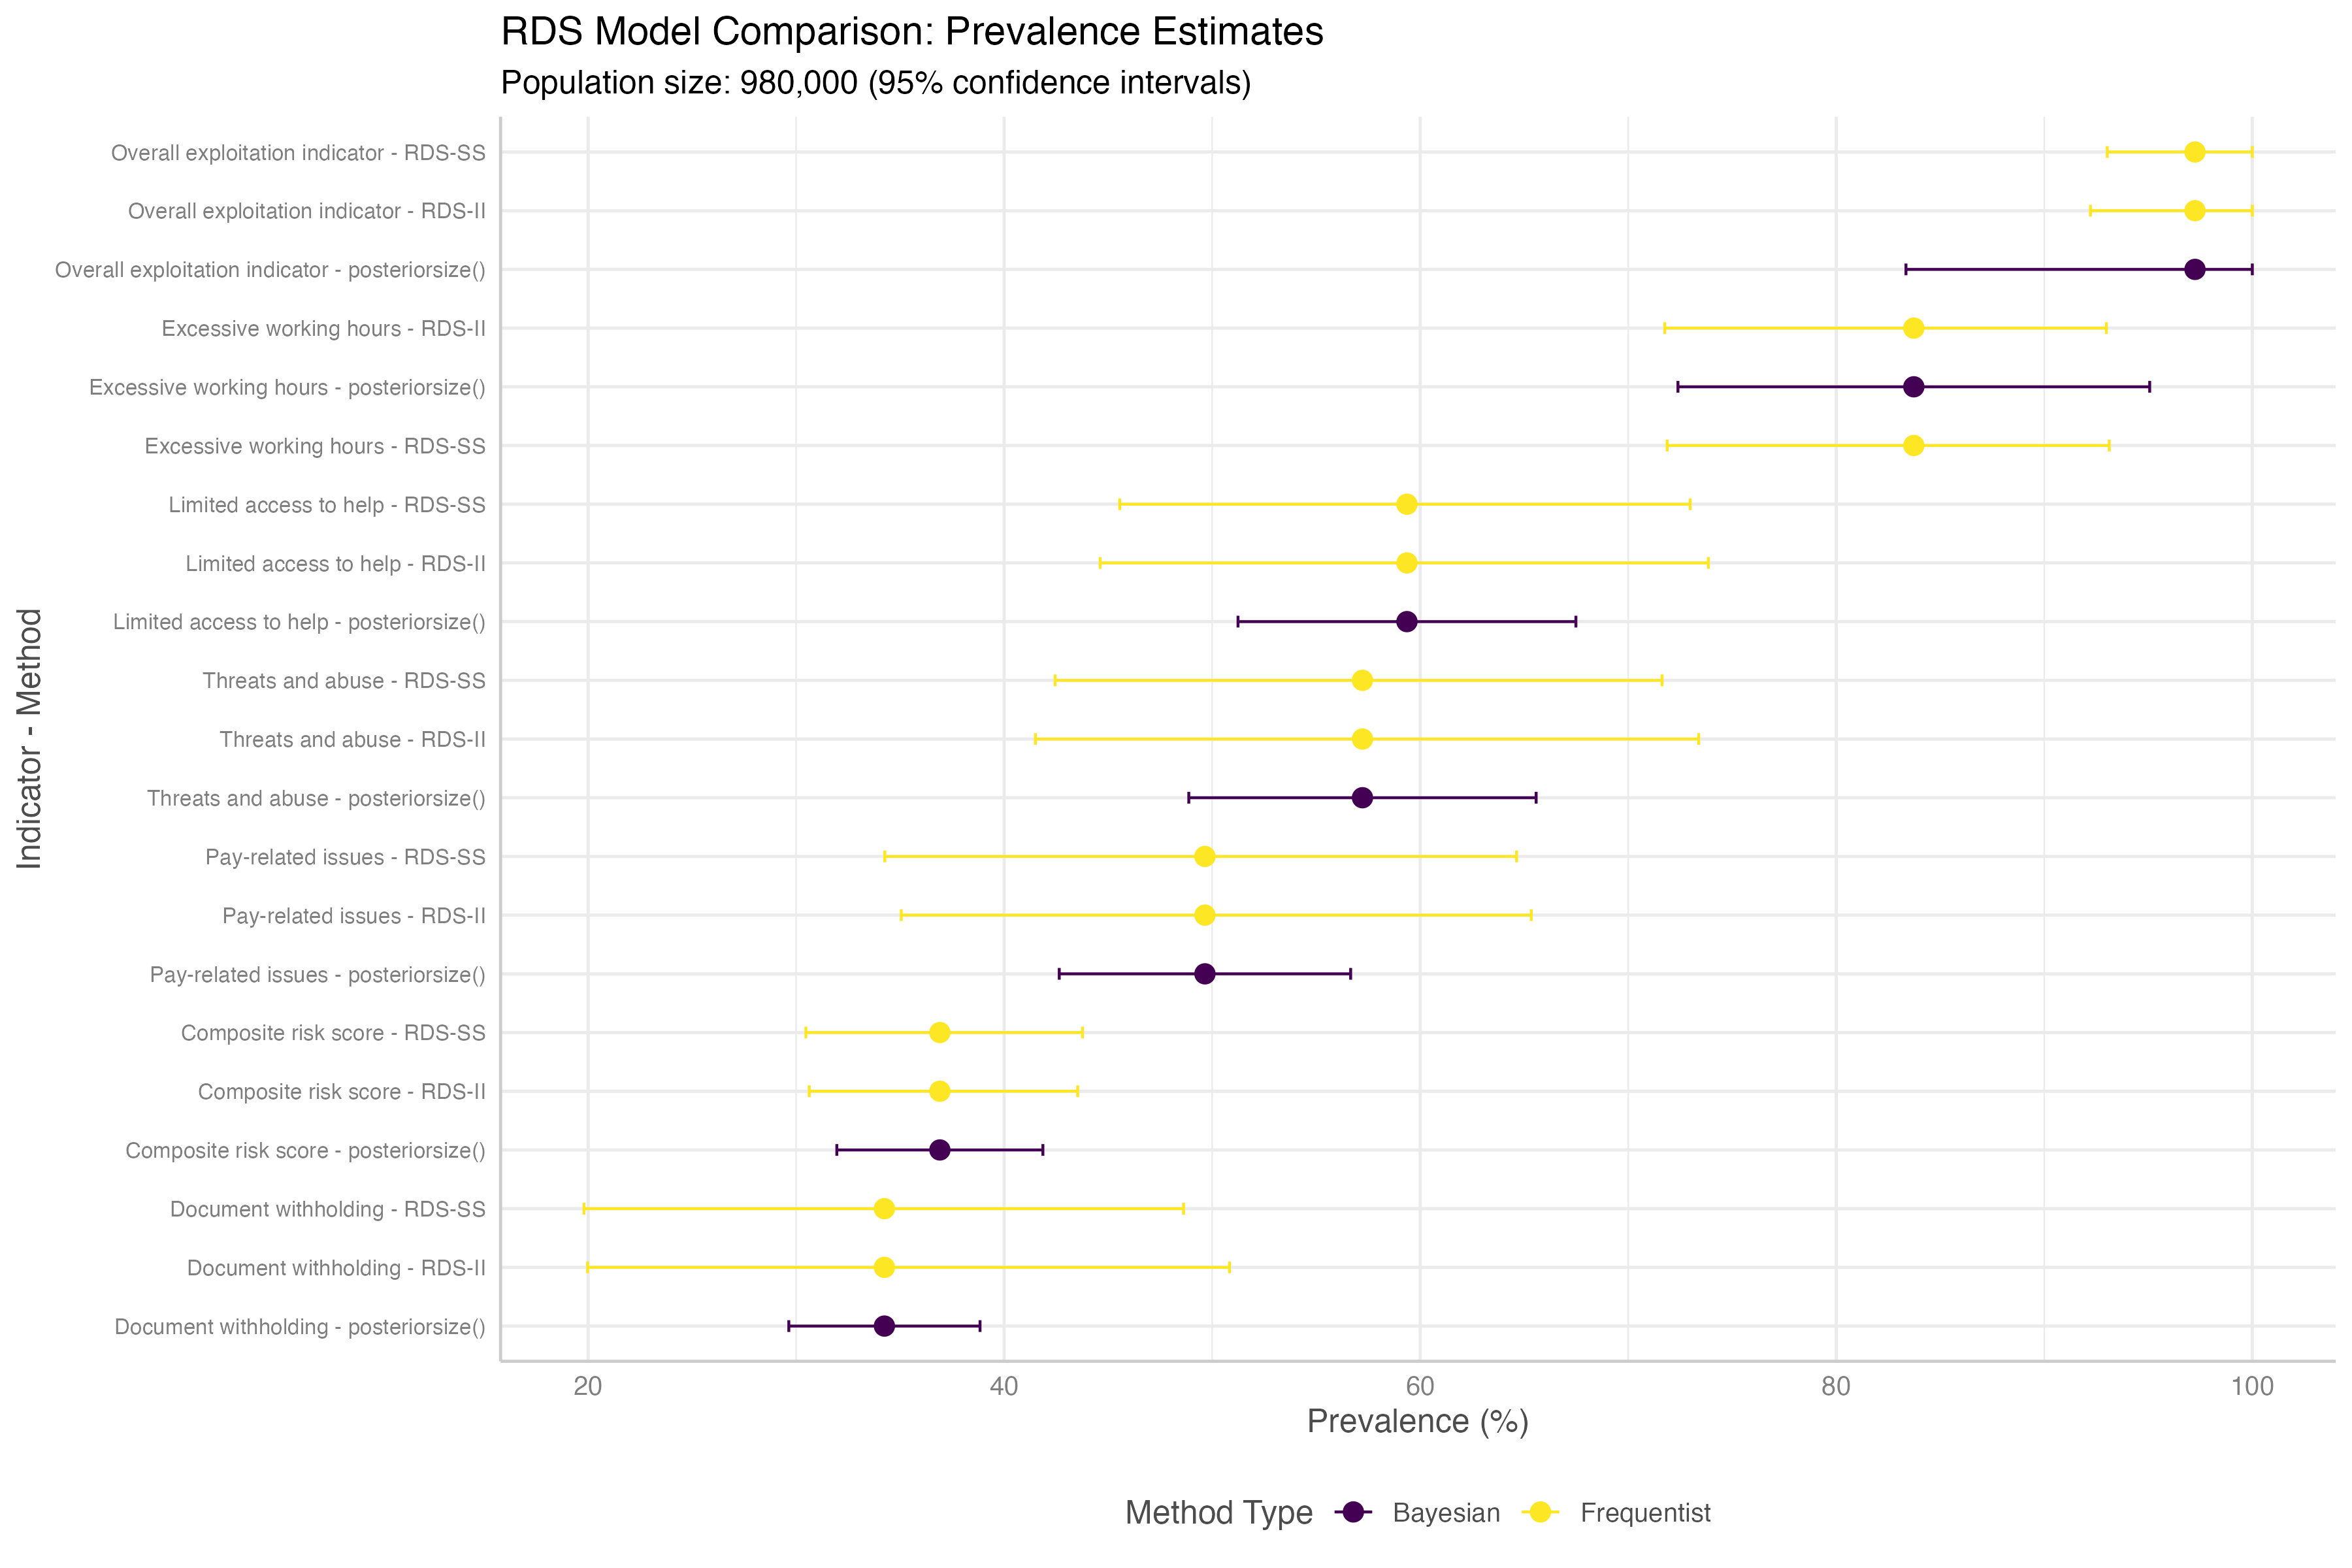
\includegraphics[width=1\linewidth,height=\textheight,keepaspectratio]{../output/figures/model_comparison_forest_plot.png}

}

\caption{\label{fig-forest-plot}Forest Plot of Exploitation Prevalence
Estimates. Comprehensive comparison of prevalence estimates across all
indicators and estimation methods, displayed as a forest plot with 95\%
confidence/credible intervals. Each row represents a different
exploitation indicator, with points showing method-specific estimates
and horizontal lines indicating uncertainty bounds. Demonstrates
consistency of findings across different analytical approaches. Source:
Authors' own work.}

\end{figure}%

\section{Discussion}\label{discussion}

\subsection{Implications for Policy}\label{implications-for-policy}

The UK Government has proved reluctant to respond to calls to remove the
restrictive, tied, visa conditions currently in force for those migrant
workers working in the UK on the Overseas Domestic Workers visa
(\textcite{gower_calls_2016}). Maintaining these restrictive conditions
prevents the ratification in the UK of C189, the International
Convention for Domestic Workers (\textcite{ILO11-indicators}). If the
estimates resulting from our study are correct, these visa conditions
place migrant domestic workers at significant risk of serious forms of
labour exploitation including, in its most severe form, exploitation
that exhibits the characteristics of forced labour---legally considered
a form of modern slavery.

To reduce the vulnerability of transnational domestic workers to
this---and other---forms of labour exploitation, we urge policy-makers
to reconsider these discriminatory visa conditions and offer the same
freedoms to domestic workers that are enjoyed by other groups of workers
under UK law.

In addition, given the vulnerabilities experienced by workers due to the
private nature of the workplace, we would urge the UK government to
consider the regulation of domestic worker employers.

Finally, given the stigma and very real danger of deportation of those
migrant domestic workers who may have fallen out of legal migration
status, our evidence suggests that there is an urgent need for the UK
Government to enforce a firewall between immigration control and labour
exploitation if the true scale of abuse is to be made visible and the
perpetrators brought to justice.

\subsection{Implications for Practice}\label{implications-for-practice}

The UK Visa and Immigration service already offers rights-based training
to migrant domestic workers via UK embassies in certain source
countries. To reduce migrant domestic workers vulnerabilities, we
advocate the expansion of this training both to include explicit
training related to employment and labour rights within the UK and to
the rapidly expanding range of new source countries from where migrant
domestic workers are now drawn.

\subsection{Methodological
Contributions}\label{methodological-contributions}

This study makes several methodological contributions to the estimation
of prevalence in hidden and hard-to-reach populations:

\textbf{Dual conceptualisation of exploitation}: We introduce two
distinct approaches to operationalising exploitation. First, we treat
exploitation as a binary outcome (exploited versus not exploited),
enabling direct comparison of prevalence estimates across RDS and NSUM
methods. Second, we construct a continuous risk index, acknowledging
that all domestic workers may be exposed to some degree of exploitation
risk. To our knowledge, this is the first application of model-assisted
RDS estimators to quantify a continuous measure of exploitation risk.

\textbf{Bayesian parameter sensitivity}:
Figure~\ref{fig-parameter-comparison} demonstrates the importance of
appropriate MCMC parameter selection for Bayesian model-assisted
estimation. Our analysis shows that enhanced parameters (featuring
longer burn-in periods and more iterations) are particularly crucial for
numeric and ordinal variables, where standard parameters may suffer from
convergence issues. This methodological innovation ensures robust
credible interval estimation for continuous risk measures.

\emph{Combining RDS and NSUM on the same survey instrument}: By
designing a survey that captures both ego and alter information, we are
able to apply RDS and NSUM to the same sample. This dual approach has
rarely been implemented in studies of labour exploitation. It provides
an opportunity to cross-validate results and assess the robustness of
prevalence estimates.

\emph{Novel bootstrap procedure for NSUM}: Recognising the non-random
nature of an RDS sample, we developed a three-step bootstrap procedure
tailored for NSUM estimation. This resamples respondents, recalculates
weights, and re-estimates NSUM prevalence at each iteration. The
procedure captures multiple layers of uncertainty and produces more
reliable confidence intervals than conventional methods, particularly in
small samples.

\emph{Application to domestic workers in the UK}: Finally, by applying
these methods to a population that is both highly stigmatised and
under-researched, we demonstrate the feasibility of using advanced
network-based estimation techniques in contexts where traditional
sampling is impossible. This methodological innovation has potential
applications in studies of other hidden labour markets and vulnerable
populations.

\subsection{Limitations of the Study}\label{limitations-of-the-study}

As with any empirical research, our study is subject to limitations. In
terms of nationality, our sample is not representative of the
demographics of those domestic workers employed on Overseas Domestic
Worker Visas in 2022 the UK. Due to the increasing number of workers on
Overseas Domestic Work visas from the Indian sub-continent, attempts
were made also to seed respondents from this community. This proved
difficult, with anecdotal information suggesting that domestic workers
from this community rarely had access to a personal mobile phone. It is
not therefore possible to infer the nature and extent of labour
exploitation within this sub-section of the domestic worker population.

As the network structure of our sample demonstrates, even with a
well-designed incentive scheme it proved difficult to recruit
respondents from these communities of domestic workers in subsequent
sampling waves in the time available. Most of our respondents are
therefore original sample members draw from the three domestic worker
communities used to seed the survey.

\subsection{Further Research}\label{further-research}

We believe that web-RDS combined with statistical estimators such as
NSUM offers an important method for the capture and comparison of
relative proportions of labour exploitation and abuse in sectors within
and beyond the UK. Network scale up methods, and potential enhancements
such as Generalised network scale up estimators offer to enhance
understanding, not least within operations and supply chain management
research, of the extent of labour exploitation in different sectors and
across industries.

\section{Conclusion}\label{conclusion}

\newpage

\newpage

\section{References}\label{references}

\printbibliography[heading=none]

\newpage

\appendix

\section{Appendix A}\label{app-a}

Population Parameters

Use \textasciitilde980,000 as UK domestic worker population estimate (EU
data)

Use 44,360 as NRM adult referrals baseline Address treatment of ``don't
know'' responses and zero network size claims Consider separate analysis
for Filipino subgroup

\subsection{The Survey}\label{the-survey}

(From codebook)

Compare corresponding survey questions between RDS and NSUM methods:

\begin{itemize}
\tightlist
\item
  Q70/Q71 (document withholding)
\item
  Q39+Q42/Q43 (pay issues)
\item
  Q45+Q47+Q48/Q49 (abuse/threats)
\item
  Q61+Q62/Q64 (excessive hours)
\item
  Q78/Q79 (access to help)
\end{itemize}

Risk Index Implementation

\begin{itemize}
\tightlist
\item
  Clean coding for 13 risk categories with proper weightings
\item
  NRM referral (0.35)
\item
  Forced labor indicators (0.55 total)
\item
  Below minimum wage (0.10)
\end{itemize}

\subsection{Data Processing}\label{app-dataprep}

The process of coding variables to make them comparable across the
Respondent-Driven Sampling (RDS) and Network Scale-Up Method (NSUM)
estimations is a multi-step procedure that moves from conceptual mapping
to specific data transformations. The core challenge is bridging the
``egocentric'' questions (about the respondent's own experiences, used
for RDS) with the network-based questions (about how many others the
respondent knows with certain experiences, used for NSUM). Yes, the
sources provide extensive detail on the coding of variables to make them
comparable for RDS and NSUM estimation. The fundamental challenge is to
create a fair comparison between the ``egocentric'' RDS questions (about
personal experience) and the broader ``how many do you know'' NSUM
questions. This was accomplished by first identifying thematic links
between questions and then implementing a specific coding scheme to
transform them into a consistent format. Conceptual Mapping of Variables
The team first identified sets of questions that cover the same
underlying themes, even if their wording differed. These ``linking''
questions were categorized by the team's confidence in their
comparability. Thematic Groups for Comparison: • Document Withholding
(Most Confident): Comparing personal experience (Q70) with knowing
others who lack access to their documents (Q71). • Pay/Debt Issues (High
Confidence): Linking personal experience with debt (Q39) and withheld
pay (Q42) to knowing others with such problems (Q43). • Threats/Abuse
(High Confidence): Aggregating personal experiences of being forced,
threatened, intimidated, or verbally abused (Q45, Q47, Q48) and
comparing them to knowing others who experienced threats or force (Q49).
• Excessive Hours (Lower Confidence): Combining questions about
inadequate weekly rest (Q61) and excessive overtime (Q62) to compare
with knowing others who face similar labor rights issues (Q64). The
confidence is lower because the NSUM question (Q64) also asks about
annual leave, which is not covered in the corresponding RDS questions. •
Access to Help (Least Confident): Matching whether the respondent
personally knows where to go for help (Q78) with knowing others who do
not (Q79). Coding and Transformation Process The conceptual mapping was
then put into practice through a detailed coding process, which is
explicitly documented in the project's R script. The primary goal was to
convert all variables into a binary (0/1) format, representing ``No'' or
``Yes'' to experiencing or knowing someone who experienced the issue.

Key Coding Steps:

\begin{enumerate}
\def\labelenumi{\arabic{enumi}.}
\tightlist
\item
  Handling Ambiguous Answers: For most RDS questions, responses like ``I
  don't know'' or ``Prefer not to say'' were recoded as NA (missing) to
  exclude them from the binary analysis.
\item
  Converting Categorical RDS Variables to Binary: Questions with
  multiple response options (e.g., ``Always,'' ``Often,'' ``Sometimes,''
  ``Never'') were recoded into a 0/1 format. For instance, for Q70
  (document withholding), the answers ``Always,'' ``Often,'' and
  ``Sometimes'' were all coded as 1 (indicating the presence of the
  issue), while ``Never'' was coded as 0.
\item
  Aggregating Multiple RDS Questions: For themes covered by multiple
  egocentric questions (like ``Threats/Abuse''), each individual
  question was first recoded into a binary 0/1 variable. These binary
  variables were then combined using a logical OR (\textbar). This means
  if a respondent answered ``Yes'' to any of the grouped questions
  (e.g., experiencing threats OR intimidation OR verbal abuse), the
  final composite RDS variable would be coded as 1. This aggregation was
  necessary to match the broader scope of the single corresponding NSUM
  question.
\item
  Converting NSUM Count Variables to Binary: The NSUM questions, which
  asked for a numerical count (e.g., ``how many do you know?''), were
  also converted to binary. If a respondent knew one or more people
  (\textgreater{} 0), their answer was coded as 1; if they knew zero, it
  remained 0. Through this systematic process of recoding, handling
  missing data, and aggregating variables, the team created a set of
  parallel binary indicators suitable for a direct comparison between
  the RDS and NSUM estimation frameworks.
\end{enumerate}

\section{Appendix B}\label{app-b}

This analysis estimates the prevalence of modern slavery among domestic
workers in the UK using multiple RDS methodologies. We examine two
primary indicators across various population size assumptions and
estimation techniques.

\subsection{Sample Characteristics}\label{sample-characteristics}

\subsubsection{Recruitment Network
Structure}\label{recruitment-network-structure}

\subsubsection{Demographic Composition}\label{demographic-composition}

\begin{figure}[H]

\centering{

\pandocbounded{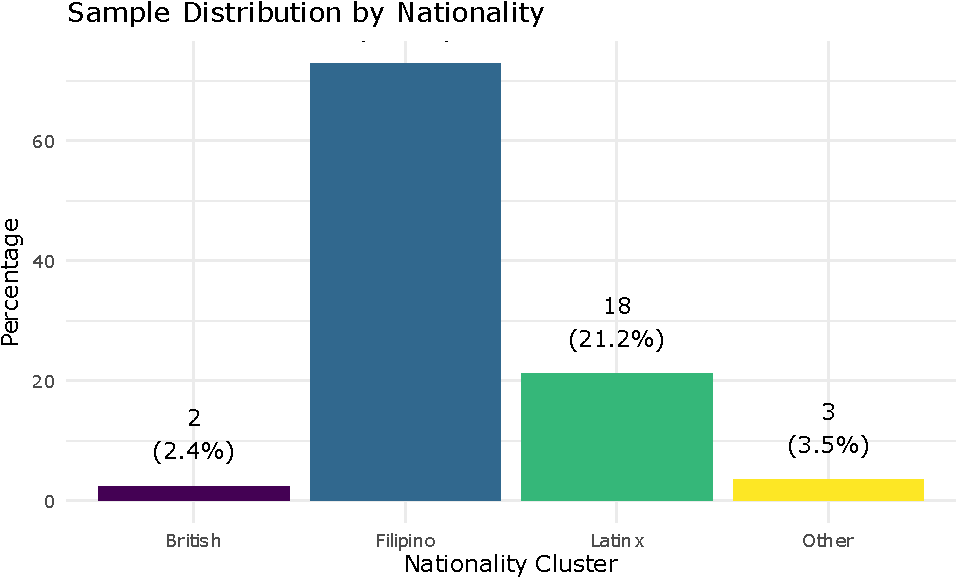
\includegraphics[keepaspectratio]{IJOPM_paperDraft_202050930_files/figure-pdf/fig-demographics-1.pdf}}

}

\caption{\label{fig-demographics}Sample Composition by Nationality
Clusters}

\end{figure}%

\subsection{RDS Estimation Results}\label{rds-estimation-results}

\subsubsection{Model-Assisted Estimates by Population
Size}\label{model-assisted-estimates-by-population-size}

\begin{table}

\caption{\label{tbl-ma-estimates}Model-Assisted Estimates by Population
Size and Seed Selection. Source: Authors' Own Work.}

\centering{

\begin{verbatim}
<div id="dtdhhlplrj" style="padding-left:0px;padding-right:0px;padding-top:10px;padding-bottom:10px;overflow-x:auto;overflow-y:auto;width:auto;height:auto;">
  <style>#dtdhhlplrj table {
  font-family: system-ui, 'Segoe UI', Roboto, Helvetica, Arial, sans-serif, 'Apple Color Emoji', 'Segoe UI Emoji', 'Segoe UI Symbol', 'Noto Color Emoji';
  -webkit-font-smoothing: antialiased;
  -moz-osx-font-smoothing: grayscale;
}

#dtdhhlplrj thead, #dtdhhlplrj tbody, #dtdhhlplrj tfoot, #dtdhhlplrj tr, #dtdhhlplrj td, #dtdhhlplrj th {
  border-style: none;
}

#dtdhhlplrj p {
  margin: 0;
  padding: 0;
}

#dtdhhlplrj .gt_table {
  display: table;
  border-collapse: collapse;
  line-height: normal;
  margin-left: auto;
  margin-right: auto;
  color: #333333;
  font-size: 9px;
  font-weight: normal;
  font-style: normal;
  background-color: #FFFFFF;
  width: 85%;
  border-top-style: solid;
  border-top-width: 2px;
  border-top-color: #A8A8A8;
  border-right-style: none;
  border-right-width: 2px;
  border-right-color: #D3D3D3;
  border-bottom-style: solid;
  border-bottom-width: 2px;
  border-bottom-color: #A8A8A8;
  border-left-style: none;
  border-left-width: 2px;
  border-left-color: #D3D3D3;
}

#dtdhhlplrj .gt_caption {
  padding-top: 4px;
  padding-bottom: 4px;
}

#dtdhhlplrj .gt_title {
  color: #333333;
  font-size: 125%;
  font-weight: initial;
  padding-top: 4px;
  padding-bottom: 4px;
  padding-left: 5px;
  padding-right: 5px;
  border-bottom-color: #FFFFFF;
  border-bottom-width: 0;
}

#dtdhhlplrj .gt_subtitle {
  color: #333333;
  font-size: 85%;
  font-weight: initial;
  padding-top: 3px;
  padding-bottom: 5px;
  padding-left: 5px;
  padding-right: 5px;
  border-top-color: #FFFFFF;
  border-top-width: 0;
}

#dtdhhlplrj .gt_heading {
  background-color: #FFFFFF;
  text-align: center;
  border-bottom-color: #FFFFFF;
  border-left-style: none;
  border-left-width: 1px;
  border-left-color: #D3D3D3;
  border-right-style: none;
  border-right-width: 1px;
  border-right-color: #D3D3D3;
}

#dtdhhlplrj .gt_bottom_border {
  border-bottom-style: solid;
  border-bottom-width: 2px;
  border-bottom-color: #D3D3D3;
}

#dtdhhlplrj .gt_col_headings {
  border-top-style: solid;
  border-top-width: 2px;
  border-top-color: #D3D3D3;
  border-bottom-style: solid;
  border-bottom-width: 2px;
  border-bottom-color: #D3D3D3;
  border-left-style: none;
  border-left-width: 1px;
  border-left-color: #D3D3D3;
  border-right-style: none;
  border-right-width: 1px;
  border-right-color: #D3D3D3;
}

#dtdhhlplrj .gt_col_heading {
  color: #333333;
  background-color: #FFFFFF;
  font-size: 8px;
  font-weight: normal;
  text-transform: inherit;
  border-left-style: none;
  border-left-width: 1px;
  border-left-color: #D3D3D3;
  border-right-style: none;
  border-right-width: 1px;
  border-right-color: #D3D3D3;
  vertical-align: bottom;
  padding-top: 5px;
  padding-bottom: 6px;
  padding-left: 5px;
  padding-right: 5px;
  overflow-x: hidden;
}

#dtdhhlplrj .gt_column_spanner_outer {
  color: #333333;
  background-color: #FFFFFF;
  font-size: 8px;
  font-weight: normal;
  text-transform: inherit;
  padding-top: 0;
  padding-bottom: 0;
  padding-left: 4px;
  padding-right: 4px;
}

#dtdhhlplrj .gt_column_spanner_outer:first-child {
  padding-left: 0;
}

#dtdhhlplrj .gt_column_spanner_outer:last-child {
  padding-right: 0;
}

#dtdhhlplrj .gt_column_spanner {
  border-bottom-style: solid;
  border-bottom-width: 2px;
  border-bottom-color: #D3D3D3;
  vertical-align: bottom;
  padding-top: 5px;
  padding-bottom: 5px;
  overflow-x: hidden;
  display: inline-block;
  width: 100%;
}

#dtdhhlplrj .gt_spanner_row {
  border-bottom-style: hidden;
}

#dtdhhlplrj .gt_group_heading {
  padding-top: 8px;
  padding-bottom: 8px;
  padding-left: 5px;
  padding-right: 5px;
  color: #333333;
  background-color: #FFFFFF;
  font-size: 100%;
  font-weight: initial;
  text-transform: inherit;
  border-top-style: solid;
  border-top-width: 2px;
  border-top-color: #D3D3D3;
  border-bottom-style: solid;
  border-bottom-width: 2px;
  border-bottom-color: #D3D3D3;
  border-left-style: none;
  border-left-width: 1px;
  border-left-color: #D3D3D3;
  border-right-style: none;
  border-right-width: 1px;
  border-right-color: #D3D3D3;
  vertical-align: middle;
  text-align: left;
}

#dtdhhlplrj .gt_empty_group_heading {
  padding: 0.5px;
  color: #333333;
  background-color: #FFFFFF;
  font-size: 100%;
  font-weight: initial;
  border-top-style: solid;
  border-top-width: 2px;
  border-top-color: #D3D3D3;
  border-bottom-style: solid;
  border-bottom-width: 2px;
  border-bottom-color: #D3D3D3;
  vertical-align: middle;
}

#dtdhhlplrj .gt_from_md > :first-child {
  margin-top: 0;
}

#dtdhhlplrj .gt_from_md > :last-child {
  margin-bottom: 0;
}

#dtdhhlplrj .gt_row {
  padding-top: 8px;
  padding-bottom: 8px;
  padding-left: 5px;
  padding-right: 5px;
  margin: 10px;
  border-top-style: solid;
  border-top-width: 1px;
  border-top-color: #D3D3D3;
  border-left-style: none;
  border-left-width: 1px;
  border-left-color: #D3D3D3;
  border-right-style: none;
  border-right-width: 1px;
  border-right-color: #D3D3D3;
  vertical-align: middle;
  overflow-x: hidden;
}

#dtdhhlplrj .gt_stub {
  color: #333333;
  background-color: #FFFFFF;
  font-size: 100%;
  font-weight: initial;
  text-transform: inherit;
  border-right-style: solid;
  border-right-width: 2px;
  border-right-color: #D3D3D3;
  padding-left: 5px;
  padding-right: 5px;
}

#dtdhhlplrj .gt_stub_row_group {
  color: #333333;
  background-color: #FFFFFF;
  font-size: 100%;
  font-weight: initial;
  text-transform: inherit;
  border-right-style: solid;
  border-right-width: 2px;
  border-right-color: #D3D3D3;
  padding-left: 5px;
  padding-right: 5px;
  vertical-align: top;
}

#dtdhhlplrj .gt_row_group_first td {
  border-top-width: 2px;
}

#dtdhhlplrj .gt_row_group_first th {
  border-top-width: 2px;
}

#dtdhhlplrj .gt_summary_row {
  color: #333333;
  background-color: #FFFFFF;
  text-transform: inherit;
  padding-top: 8px;
  padding-bottom: 8px;
  padding-left: 5px;
  padding-right: 5px;
}

#dtdhhlplrj .gt_first_summary_row {
  border-top-style: solid;
  border-top-color: #D3D3D3;
}

#dtdhhlplrj .gt_first_summary_row.thick {
  border-top-width: 2px;
}

#dtdhhlplrj .gt_last_summary_row {
  padding-top: 8px;
  padding-bottom: 8px;
  padding-left: 5px;
  padding-right: 5px;
  border-bottom-style: solid;
  border-bottom-width: 2px;
  border-bottom-color: #D3D3D3;
}

#dtdhhlplrj .gt_grand_summary_row {
  color: #333333;
  background-color: #FFFFFF;
  text-transform: inherit;
  padding-top: 8px;
  padding-bottom: 8px;
  padding-left: 5px;
  padding-right: 5px;
}

#dtdhhlplrj .gt_first_grand_summary_row {
  padding-top: 8px;
  padding-bottom: 8px;
  padding-left: 5px;
  padding-right: 5px;
  border-top-style: double;
  border-top-width: 6px;
  border-top-color: #D3D3D3;
}

#dtdhhlplrj .gt_last_grand_summary_row_top {
  padding-top: 8px;
  padding-bottom: 8px;
  padding-left: 5px;
  padding-right: 5px;
  border-bottom-style: double;
  border-bottom-width: 6px;
  border-bottom-color: #D3D3D3;
}

#dtdhhlplrj .gt_striped {
  background-color: rgba(128, 128, 128, 0.05);
}

#dtdhhlplrj .gt_table_body {
  border-top-style: solid;
  border-top-width: 2px;
  border-top-color: #D3D3D3;
  border-bottom-style: solid;
  border-bottom-width: 2px;
  border-bottom-color: #D3D3D3;
}

#dtdhhlplrj .gt_footnotes {
  color: #333333;
  background-color: #FFFFFF;
  border-bottom-style: none;
  border-bottom-width: 2px;
  border-bottom-color: #D3D3D3;
  border-left-style: none;
  border-left-width: 2px;
  border-left-color: #D3D3D3;
  border-right-style: none;
  border-right-width: 2px;
  border-right-color: #D3D3D3;
}

#dtdhhlplrj .gt_footnote {
  margin: 0px;
  font-size: 90%;
  padding-top: 4px;
  padding-bottom: 4px;
  padding-left: 5px;
  padding-right: 5px;
}

#dtdhhlplrj .gt_sourcenotes {
  color: #333333;
  background-color: #FFFFFF;
  border-bottom-style: none;
  border-bottom-width: 2px;
  border-bottom-color: #D3D3D3;
  border-left-style: none;
  border-left-width: 2px;
  border-left-color: #D3D3D3;
  border-right-style: none;
  border-right-width: 2px;
  border-right-color: #D3D3D3;
}

#dtdhhlplrj .gt_sourcenote {
  font-size: 90%;
  padding-top: 4px;
  padding-bottom: 4px;
  padding-left: 5px;
  padding-right: 5px;
}

#dtdhhlplrj .gt_left {
  text-align: left;
}

#dtdhhlplrj .gt_center {
  text-align: center;
}

#dtdhhlplrj .gt_right {
  text-align: right;
  font-variant-numeric: tabular-nums;
}

#dtdhhlplrj .gt_font_normal {
  font-weight: normal;
}

#dtdhhlplrj .gt_font_bold {
  font-weight: bold;
}

#dtdhhlplrj .gt_font_italic {
  font-style: italic;
}

#dtdhhlplrj .gt_super {
  font-size: 65%;
}

#dtdhhlplrj .gt_footnote_marks {
  font-size: 75%;
  vertical-align: 0.4em;
  position: initial;
}

#dtdhhlplrj .gt_asterisk {
  font-size: 100%;
  vertical-align: 0;
}

#dtdhhlplrj .gt_indent_1 {
  text-indent: 5px;
}

#dtdhhlplrj .gt_indent_2 {
  text-indent: 10px;
}

#dtdhhlplrj .gt_indent_3 {
  text-indent: 15px;
}

#dtdhhlplrj .gt_indent_4 {
  text-indent: 20px;
}

#dtdhhlplrj .gt_indent_5 {
  text-indent: 25px;
}

#dtdhhlplrj .katex-display {
  display: inline-flex !important;
  margin-bottom: 0.75em !important;
}

#dtdhhlplrj div.Reactable > div.rt-table > div.rt-thead > div.rt-tr.rt-tr-group-header > div.rt-th-group:after {
  height: 0px !important;
}
</style>
  <table class="gt_table" data-quarto-disable-processing="false" data-quarto-bootstrap="false">
  <thead>
    <tr class="gt_heading">
      <td colspan="6" class="gt_heading gt_title gt_font_normal gt_bottom_border" style>Model-Assisted Estimates by Population Size and Seed Selection</td>
    </tr>
    
    <tr class="gt_col_headings gt_spanner_row">
      <th class="gt_col_heading gt_columns_bottom_border gt_left" rowspan="2" colspan="1" scope="col" id="seed_method">Seed Selection</th>
      <th class="gt_col_heading gt_columns_bottom_border gt_right" rowspan="2" colspan="1" scope="col" id="pop_size_f">Population Size</th>
      <th class="gt_center gt_columns_top_border gt_column_spanner_outer" rowspan="1" colspan="4" scope="colgroup" id="Prevalence Estimates (95% CI)">
        <div class="gt_column_spanner">Prevalence Estimates (95% CI)</div>
      </th>
    </tr>
    <tr class="gt_col_headings">
      <th class="gt_col_heading gt_columns_bottom_border gt_right" rowspan="1" colspan="1" scope="col" id="Document-Withholding">Document Withholding</th>
      <th class="gt_col_heading gt_columns_bottom_border gt_right" rowspan="1" colspan="1" scope="col" id="Pay-Issues">Pay Issues</th>
      <th class="gt_col_heading gt_columns_bottom_border gt_right" rowspan="1" colspan="1" scope="col" id="Excessive-Hours">Excessive Hours</th>
      <th class="gt_col_heading gt_columns_bottom_border gt_right" rowspan="1" colspan="1" scope="col" id="Threats/Abuse">Threats/Abuse</th>
    </tr>
  </thead>
  <tbody class="gt_table_body">
    <tr><td headers="seed_method" class="gt_row gt_left">sample</td>
<td headers="pop_size_f" class="gt_row gt_right">50,000</td>
<td headers="Document Withholding" class="gt_row gt_right">34.1% (16.1%, 52.1%)</td>
<td headers="Pay Issues" class="gt_row gt_right">49.3% (35.2%, 63.4%)</td>
<td headers="Excessive Hours" class="gt_row gt_right">84.0% (72.3%, 95.8%)</td>
<td headers="Threats/Abuse" class="gt_row gt_right">57.1% (34.6%, 79.6%)</td></tr>
    <tr><td headers="seed_method" class="gt_row gt_left">sample</td>
<td headers="pop_size_f" class="gt_row gt_right">980,000</td>
<td headers="Document Withholding" class="gt_row gt_right">34.3% (16.4%, 52.2%)</td>
<td headers="Pay Issues" class="gt_row gt_right">49.5% (35.6%, 63.5%)</td>
<td headers="Excessive Hours" class="gt_row gt_right">83.7% (71.9%, 95.6%)</td>
<td headers="Threats/Abuse" class="gt_row gt_right">57.3% (35.4%, 79.3%)</td></tr>
    <tr><td headers="seed_method" class="gt_row gt_left">sample</td>
<td headers="pop_size_f" class="gt_row gt_right">1,740,000</td>
<td headers="Document Withholding" class="gt_row gt_right">34.3% (16.0%, 52.7%)</td>
<td headers="Pay Issues" class="gt_row gt_right">49.1% (34.9%, 63.3%)</td>
<td headers="Excessive Hours" class="gt_row gt_right">83.8% (72.1%, 95.6%)</td>
<td headers="Threats/Abuse" class="gt_row gt_right">57.0% (34.7%, 79.3%)</td></tr>
    <tr><td headers="seed_method" class="gt_row gt_left">random</td>
<td headers="pop_size_f" class="gt_row gt_right">50,000</td>
<td headers="Document Withholding" class="gt_row gt_right">34.1% (16.1%, 52.1%)</td>
<td headers="Pay Issues" class="gt_row gt_right">49.3% (35.2%, 63.4%)</td>
<td headers="Excessive Hours" class="gt_row gt_right">84.0% (72.3%, 95.8%)</td>
<td headers="Threats/Abuse" class="gt_row gt_right">57.1% (34.6%, 79.6%)</td></tr>
    <tr><td headers="seed_method" class="gt_row gt_left">random</td>
<td headers="pop_size_f" class="gt_row gt_right">980,000</td>
<td headers="Document Withholding" class="gt_row gt_right">34.3% (16.4%, 52.2%)</td>
<td headers="Pay Issues" class="gt_row gt_right">49.5% (35.6%, 63.5%)</td>
<td headers="Excessive Hours" class="gt_row gt_right">83.7% (71.9%, 95.6%)</td>
<td headers="Threats/Abuse" class="gt_row gt_right">57.3% (35.4%, 79.3%)</td></tr>
    <tr><td headers="seed_method" class="gt_row gt_left">random</td>
<td headers="pop_size_f" class="gt_row gt_right">1,740,000</td>
<td headers="Document Withholding" class="gt_row gt_right">34.3% (16.0%, 52.7%)</td>
<td headers="Pay Issues" class="gt_row gt_right">49.1% (34.9%, 63.3%)</td>
<td headers="Excessive Hours" class="gt_row gt_right">83.8% (72.1%, 95.6%)</td>
<td headers="Threats/Abuse" class="gt_row gt_right">57.0% (34.7%, 79.3%)</td></tr>
    <tr><td headers="seed_method" class="gt_row gt_left">degree</td>
<td headers="pop_size_f" class="gt_row gt_right">50,000</td>
<td headers="Document Withholding" class="gt_row gt_right">34.1% (16.1%, 52.1%)</td>
<td headers="Pay Issues" class="gt_row gt_right">49.3% (35.2%, 63.4%)</td>
<td headers="Excessive Hours" class="gt_row gt_right">84.0% (72.3%, 95.8%)</td>
<td headers="Threats/Abuse" class="gt_row gt_right">57.1% (34.6%, 79.6%)</td></tr>
    <tr><td headers="seed_method" class="gt_row gt_left">degree</td>
<td headers="pop_size_f" class="gt_row gt_right">980,000</td>
<td headers="Document Withholding" class="gt_row gt_right">34.3% (16.4%, 52.2%)</td>
<td headers="Pay Issues" class="gt_row gt_right">49.5% (35.6%, 63.5%)</td>
<td headers="Excessive Hours" class="gt_row gt_right">83.7% (71.9%, 95.6%)</td>
<td headers="Threats/Abuse" class="gt_row gt_right">57.3% (35.4%, 79.3%)</td></tr>
    <tr><td headers="seed_method" class="gt_row gt_left">degree</td>
<td headers="pop_size_f" class="gt_row gt_right">1,740,000</td>
<td headers="Document Withholding" class="gt_row gt_right">34.3% (16.0%, 52.7%)</td>
<td headers="Pay Issues" class="gt_row gt_right">49.1% (34.9%, 63.3%)</td>
<td headers="Excessive Hours" class="gt_row gt_right">83.8% (72.1%, 95.6%)</td>
<td headers="Threats/Abuse" class="gt_row gt_right">57.0% (34.7%, 79.3%)</td></tr>
  </tbody>
  
  
</table>
</div>
\end{verbatim}

}

\end{table}%

\subsubsection{Traditional RDS Estimators
Comparison}\label{traditional-rds-estimators-comparison}

\begin{table}

\caption{\label{tbl-rds-comparison}RDS Estimator Comparison for Binary
Indicators. Source: Authors' Own Work.}

\centering{

\begin{verbatim}
NULL
\end{verbatim}

}

\end{table}%

\subsection{Subgroup Analysis}\label{subgroup-analysis}

\begin{longtable}[t]{lllrr}
\caption{\label{tab:netclust-analysis}Clustered SS-PSE prevalence estimates for labour
exploitation indicators among domestic workers}\\
\toprule
 & Indicator & Prevalence (95\% CI) & Sample with trait & Total sample\\
\midrule
\cellcolor{gray!10}{97.5\%} & \cellcolor{gray!10}{Document withholding} & \cellcolor{gray!10}{0.08\% (0.017–0.693\%)} & \cellcolor{gray!10}{22} & \cellcolor{gray!10}{85}\\
97.5\%1 & Pay-related issues & 0.209\% (0.043–1.556\%) & 48 & 85\\
\cellcolor{gray!10}{97.5\%2} & \cellcolor{gray!10}{Threats/abuse} & \cellcolor{gray!10}{0.2\% (0.042–1.733\%)} & \cellcolor{gray!10}{51} & \cellcolor{gray!10}{85}\\
97.5\%3 & Excessive hours & 0.276\% (0.056–2.744\%) & 70 & 85\\
\cellcolor{gray!10}{97.5\%4} & \cellcolor{gray!10}{Limited access to help} & \cellcolor{gray!10}{0.205\% (0.039–1.666\%)} & \cellcolor{gray!10}{49} & \cellcolor{gray!10}{85}\\
\bottomrule
\multicolumn{5}{l}{\rule{0pt}{1em}\textit{Note: }}\\
\multicolumn{5}{l}{\rule{0pt}{1em}makecell[l]{Estimates based on Clustered Sequential Sampling\Population Size Estimation (Clustered SS-PSE) methodology using netclust\package. Population size assumption: 980,000 UK domestic workers.\Confidence intervals derived from MCMC sampling (1,000 samples, 2,000\burn-in). Analysis accounts for nationality clustering (Filipino, Latinx,\Other Combined) and network structure in RDS data.}}\\
\end{longtable}

Clustered SS-PSE prevalence estimates for labour exploitation indicators

\begin{figure}[H]

{\centering \pandocbounded{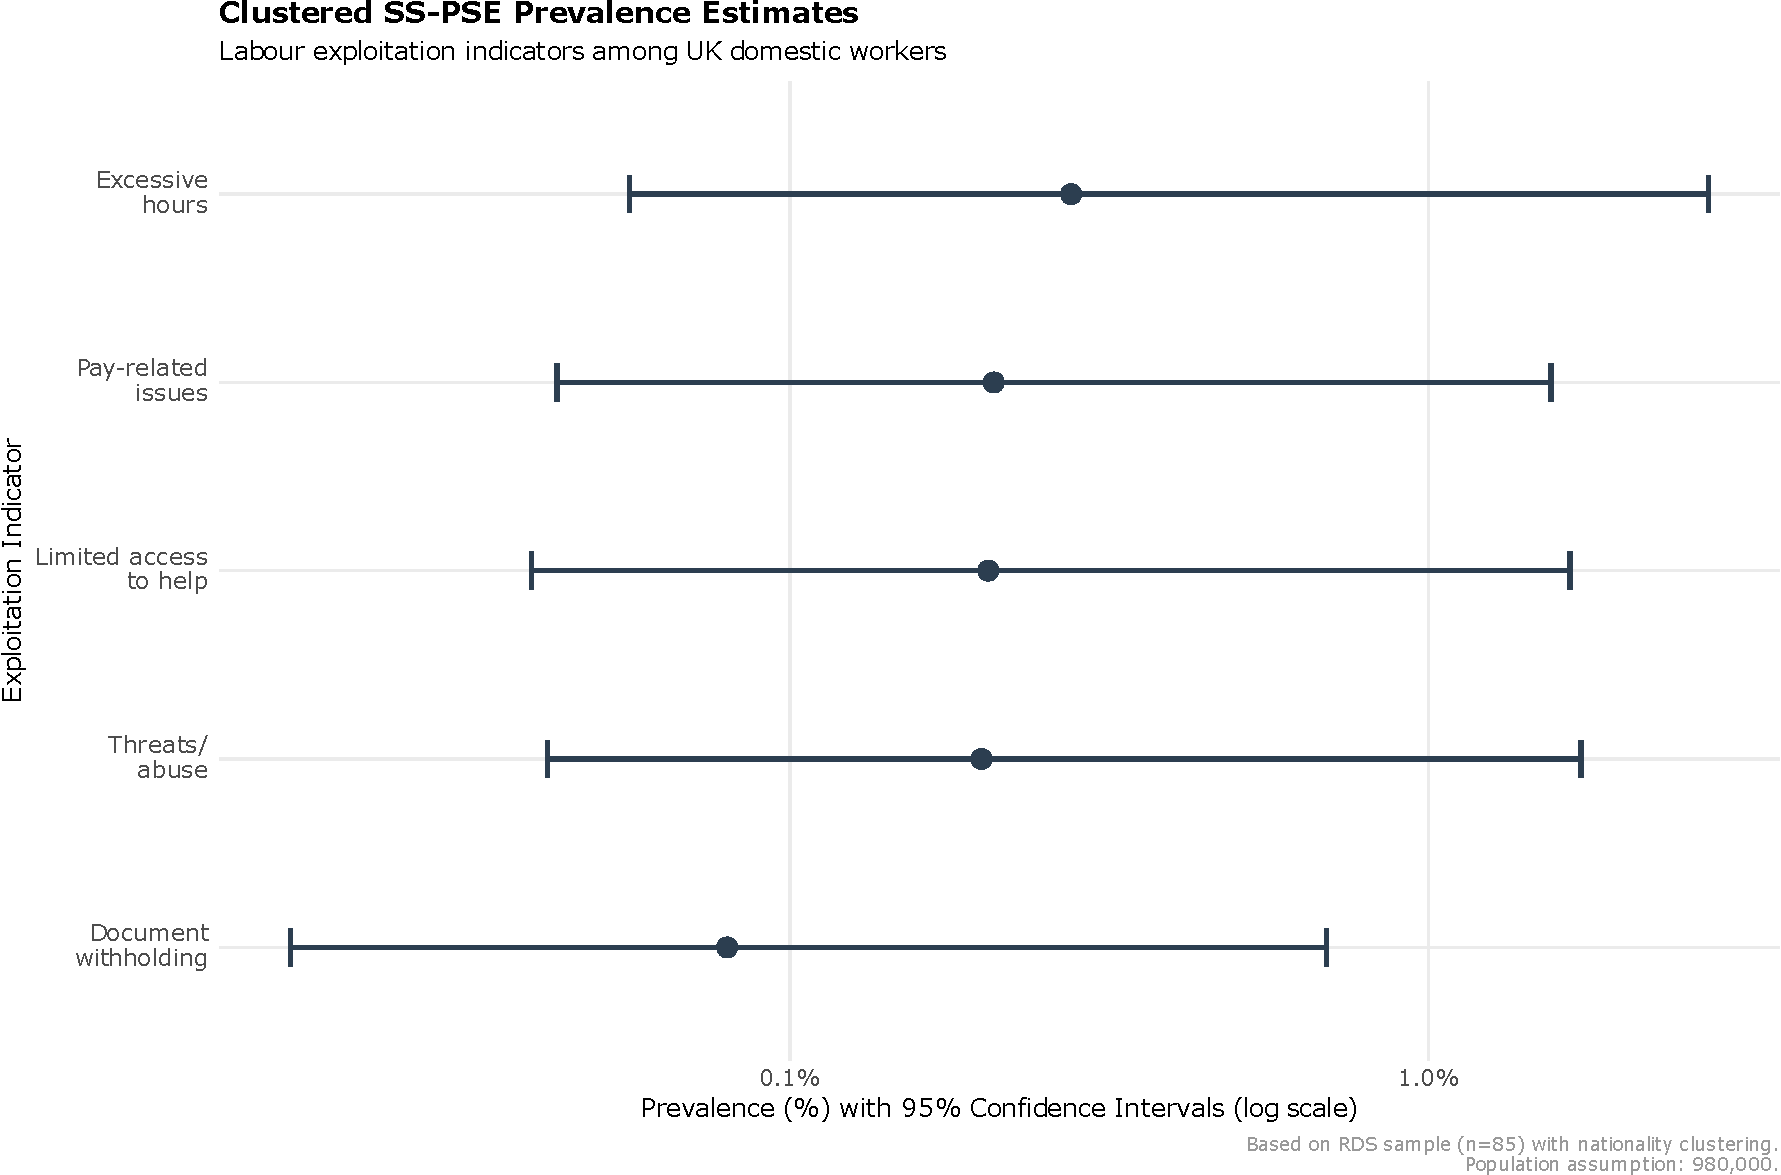
\includegraphics[keepaspectratio]{IJOPM_paperDraft_202050930_files/figure-pdf/netclust-analysis-1.pdf}}

}

\caption{Clustered SS-PSE prevalence estimates for labour exploitation
indicators}

\end{figure}%

\begin{figure}[H]

{\centering \pandocbounded{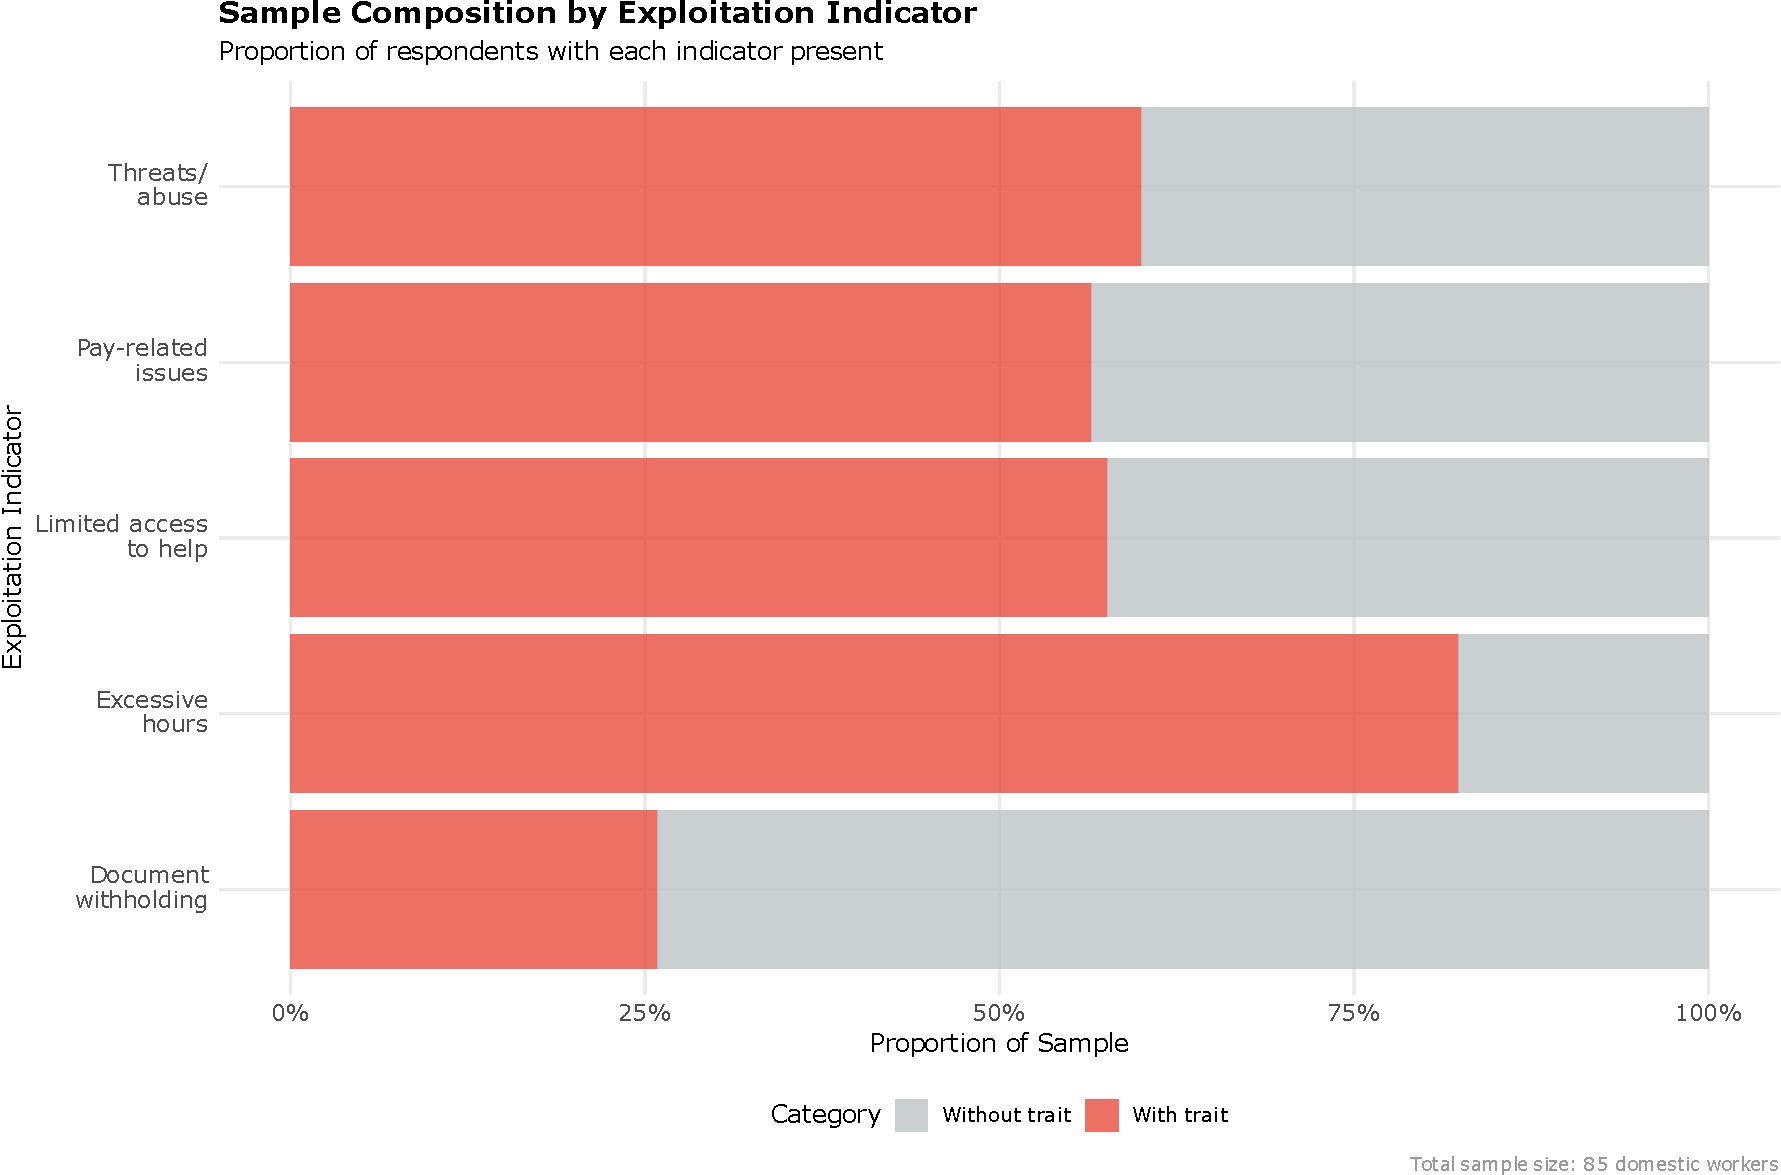
\includegraphics[keepaspectratio]{IJOPM_paperDraft_202050930_files/figure-pdf/netclust-analysis-2.pdf}}

}

\caption{Clustered SS-PSE prevalence estimates for labour exploitation
indicators}

\end{figure}%

\begin{figure}[H]

{\centering \pandocbounded{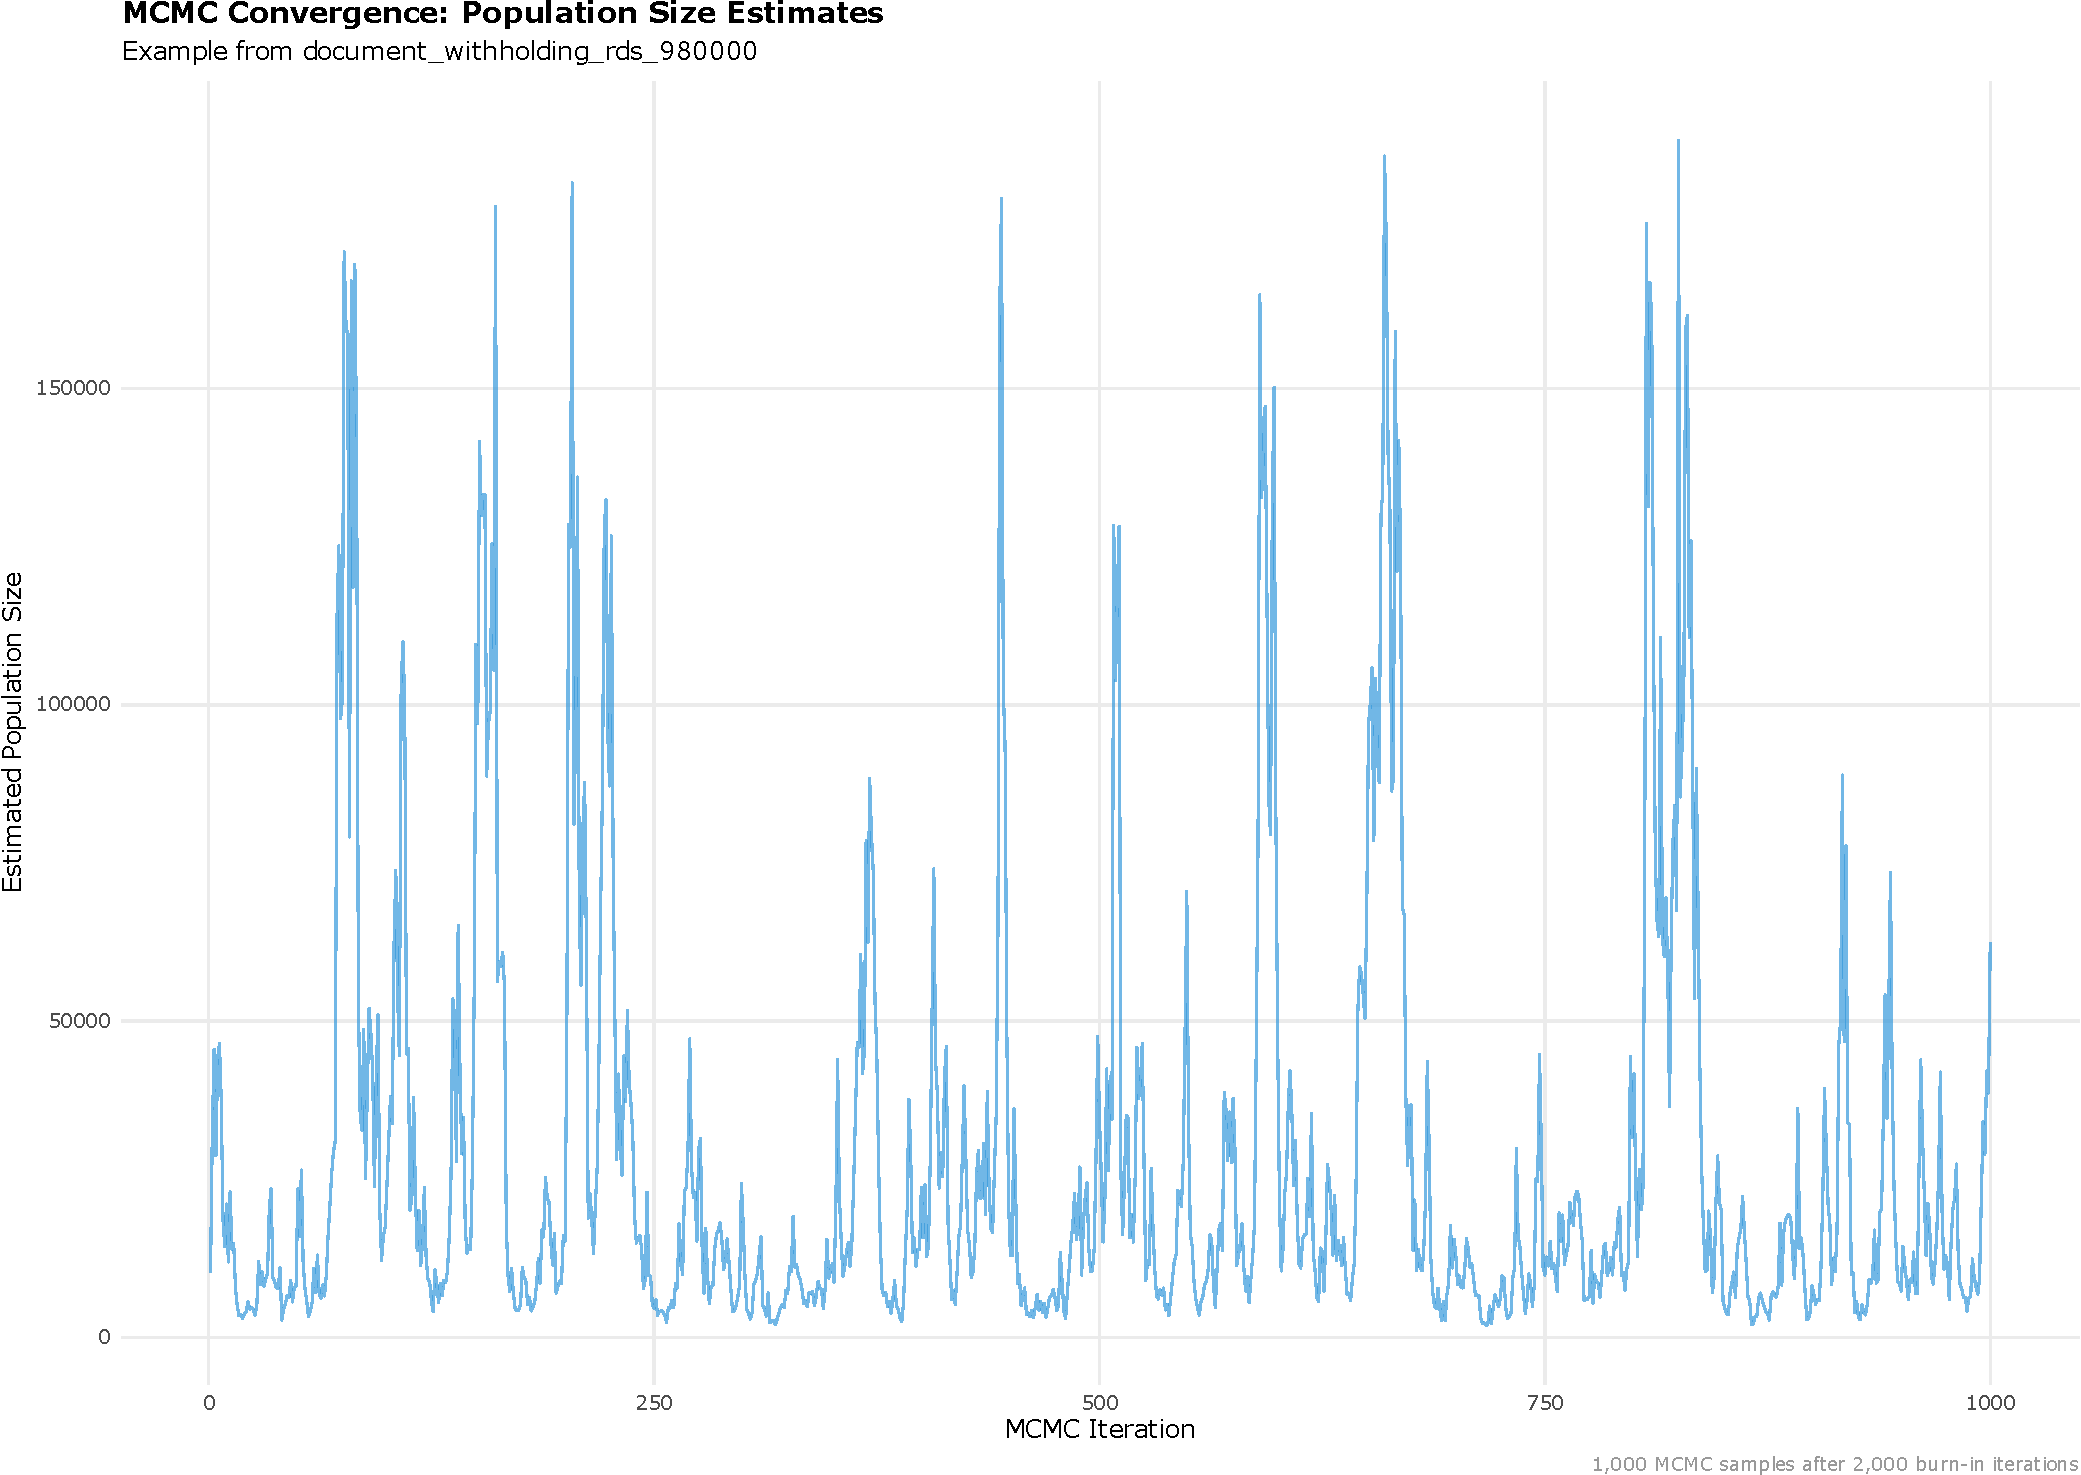
\includegraphics[keepaspectratio]{IJOPM_paperDraft_202050930_files/figure-pdf/netclust-analysis-3.pdf}}

}

\caption{Clustered SS-PSE prevalence estimates for labour exploitation
indicators}

\end{figure}%

\begin{verbatim}

=== NETCLUST ANALYSIS SUMMARY ===
\end{verbatim}

\begin{verbatim}
Analysis Configuration:
\end{verbatim}

\begin{verbatim}
- Population size assumption: 980,000 UK
domestic workers
\end{verbatim}

\begin{verbatim}
- MCMC samples: 1000 
\end{verbatim}

\begin{verbatim}
- Burn-in iterations: 2000 
\end{verbatim}

\begin{verbatim}
- Number of nationality clusters: 3 
\end{verbatim}

\begin{verbatim}
- Total sample size: 85 
\end{verbatim}

\begin{verbatim}

Cluster composition:
\end{verbatim}

\begin{verbatim}
- Filipino : 62 respondents
- Latinx : 18 respondents
- Other Combined : 5 respondents
\end{verbatim}

\begin{verbatim}

Key Findings:
\end{verbatim}

\begin{verbatim}
- Highest prevalence: Excessive hours (0.3%)
\end{verbatim}

\begin{verbatim}
- Lowest prevalence: Document withholding (0.1%)
\end{verbatim}

\begin{verbatim}
- All estimates show successful MCMC convergence
\end{verbatim}

\begin{verbatim}
- Wide confidence intervals reflect uncertainty in hidden population
estimation
\end{verbatim}

\section{Appendix C: Bootstrap Estimation for Network Scale-Up Using RDS
Data}\label{app-3step}

\subsection{Introduction}\label{introduction-1}

When estimating the size or characteristics of a hidden population using
the Network Scale-Up Method (NSUM), researchers typically assume a
probability sample from the frame population. However, in many applied
settings---including hard-to-reach populations---data are collected
via*Respondent-Driven Sampling (RDS). RDS introduces specific structural
dependencies and inclusion probabilities that violate the assumptions of
simple random sampling.

This presents a challenge: how can we correctly estimate uncertainty for
NSUM estimates derived from an RDS sample? As shown in
\textcite{feeh16-generalized} and \textcite{salg06-variance}, the NSUM
estimator depends crucially on inclusion weights \(\pi_i\), which must
reflect the sampling design. When data are RDS-based, these weights are
typically derived from known degree-based estimators such as RDS-II or
Gile's Successive Sampling (SS) weights.

To address this challenge, we propose a \textbf{three-step bootstrap
procedure} for NSUM estimation using RDS data. This approach is
flexible, modular, and applicable across several classes of NSUM
estimators. It separates the issues of: 1. How to resample an RDS chain
(Step 1), 2. How to recalculate sample-specific weights (Step 2), and 3.
How to apply a chosen NSUM estimator (Step 3).

\begin{center}\rule{0.5\linewidth}{0.5pt}\end{center}

\subsection{Step 1: Resampling the RDS
Sample}\label{step-1-resampling-the-rds-sample}

We begin by resampling from the observed RDS sample in a way that mimics
the original recruitment structure. Let the original sample be: \[
\mathcal{S} = \{i_1, i_2, \dots, i_n\}
\] with recruitment chains and wave indicators. Let \(d_i\) denote
self-reported degree for respondent \(i\), and let the recruitment tree
structure be encoded via seed/recruiter IDs.

\subsubsection{Options for RDS
Resampling}\label{options-for-rds-resampling}

\begin{itemize}
\tightlist
\item
  \textbf{Tree Bootstrap}: Sample entire recruitment trees (originating
  from seeds) with replacement. This respects the hierarchical
  recruitment structure and allows design effect estimation
  \autocite{salg06-variance}.
\item
  \textbf{Successive Sampling Bootstrap (SSB)}: Sample with replacement
  according to inclusion probabilities derived from the SS model
  (\textcite{gile11-improv}).
\item
  \textbf{Neighborhood Bootstrap}: Use ego-network topology to preserve
  recruitment ties and neighborhood structure
  (\textcite{yauc22-neighboor}).
\item
  \textbf{Chain Bootstrap:} Each bootstrap replicate samples chains or
  subchains with replacement, preserving recruiter--recruitee links.
  This is implemented in \texttt{surveybootstrap::rds.boot.draw.chain()}
  and used in studies like \textcite{weir12-comparison}.
\end{itemize}

Let \(\mathcal{S}^{(b)}\) denote the sample drawn in bootstrap replicate
\(b\).

\begin{center}\rule{0.5\linewidth}{0.5pt}\end{center}

\subsection{Step 2: Recalculating
Weights}\label{step-2-recalculating-weights}

NSUM estimators require inclusion weights \(\pi_i\) or their inverses
\(w_i = 1 / \pi_i\). Because bootstrap samples differ in composition and
recruitment pattern, these weights must be \textbf{recomputed for each
replicate}.

\subsubsection{General Structure}\label{general-structure}

For each replicate \(b\), construct: - \(\mathcal{S}^{(b)}\): resampled
respondent IDs - \(d_i^{(b)}\): degree reports in replicate -
\(\pi_i^{(b)}\): estimated inclusion probabilities

\subsubsection{Weighting Options}\label{weighting-options}

\begin{itemize}
\item
  \textbf{RDS-II Weights} (\textcite{volz08-simple}): \[
  w_i^{(b)} \propto \frac{1}{d_i^{(b)}}
  \]
\item
  \textbf{SS Weights} (\textcite{gile11-improv}): Incorporate sampling
  fraction and frame size \(N_F\). Computed numerically via successive
  sampling approximation.
\end{itemize}

Let \(\mathbf{X}_i\) denote covariates (e.g.~traits, degree, indicator
of hidden population membership), which are retained from the original
data and passed to Step 3.

\begin{center}\rule{0.5\linewidth}{0.5pt}\end{center}

\subsection{Step 3: NSUM Estimation}\label{step-3-nsum-estimation}

\subsubsection{Step 3: NSUM Estimation on Resampled and Reweighted
Data}\label{step-3-nsum-estimation-on-resampled-and-reweighted-data}

Given a bootstrap sample \(\mathcal{S}^{(b)}\), we estimate the size of
the hidden population \(N_H\) using one of several NSUM estimators. All
estimators rely on weighted sums of out-reports and degree.

\paragraph{(a) Generalized NSUM (GNSUM)}\label{a-generalized-nsum-gnsum}

As described in \textcite{feeh16-generaling}, GNSUM estimates:

\[\hat{N}_H^{(b)} = \left( \frac{\sum_{i} \frac{y_{i,H}}{\pi_i^{(b)}}}{\sum_{i} \frac{d_i}{\pi_i^{(b)}}} \right) \cdot N_F\]

Where:

\begin{itemize}
\item
  \(y_{i,H}\): number of known alters in the hidden population,
\item
  \(d_i\): degree (known network size, e.g.~from Q13),
\item
  \(N_F\): size of the frame population (e.g.~domestic workers in UK).
\end{itemize}

\paragraph{(b) GNSUM with Symmetric Visibility (for Hidden Members in
RDS)}\label{b-gnsum-with-symmetric-visibility-for-hidden-members-in-rds}

In your context, some RDS respondents are ex post identified as members
of the hidden population. Under the \textbf{symmetric visibility
assumption}, if \(i \in H\), we assume the probability that \(i\) knows
\(j\) is the same as \(j\) knows \(i\). This allows \textbf{in-reports}
to be incorporated.

Let:

\begin{itemize}
\item
  \(I_H(i) = 1\) if \(i \in H\), 0 otherwise
\item
  \(y_{i}^{\text{in}}\): number of other hidden members who report
  knowing \(i\)
\end{itemize}

Then the estimator becomes:

\[\hat{N}_H^{(b)} = \left( \frac{\sum_{i} \frac{y_{i,H} + I_H(i) \cdot y_{i}^{\text{in}}}{\pi_i^{(b)}}}{\sum_{i} \frac{d_i}{\pi_i^{(b)}}} \right) \cdot N_F\]

\paragraph{(c) Modified Basic Scale-Up
(MBSU)}\label{c-modified-basic-scale-up-mbsu}

This estimator adjusts for key reporting biases via three correction
factors:

\[\hat{N}_H^{(b)} = \left( \frac{\sum_{i} \frac{y_{i,H}}{\pi_i^{(b)}}}{\sum_{i} \frac{d_i}{\pi_i^{(b)}}} \right) \cdot N_F \cdot \frac{1}{\delta \cdot \tau \cdot \rho}\]

Where:

\begin{itemize}
\item
  \(\delta\): \textbf{Transmission bias} (probability respondent is
  aware of alter's status),
\item
  \(\tau\): \textbf{Barrier effect} (social mixing between hidden and
  frame population),
\item
  \(\rho\): \textbf{Popularity bias} (relative visibility of hidden
  population members).
\end{itemize}

These values can be:

\begin{itemize}
\item
  Estimated using \textbf{known subpopulations} (e.g., alter groups with
  known size),
\item
  Set by expert \textbf{elicitation},
\item
  Scanned in \textbf{sensitivity analysis}.
\end{itemize}

\paragraph{(d) Model-Based NSUM}\label{d-model-based-nsum}

Bayesian implementations (e.g. \textcite{malt15-estimating}) model:

\begin{itemize}
\item
  Degree distributions,
\item
  Reporting error,
\item
  Group visibility,
\item
  Hidden population size.
\end{itemize}

They yield a \textbf{posterior distribution} over \(N_H\), and
uncertainty is embedded within the model.

\begin{center}\rule{0.5\linewidth}{0.5pt}\end{center}

This step applies an NSUM estimator to the bootstrap sample
\(\mathcal{S}^{(b)}\) using the recalculated weights \(w_i^{(b)}\) and
responses \(y_{i,H}\), where \(y_{i,H}\) is the number of known contacts
respondent \(i\) has in hidden population \(H\).

Let \(N_F\) denote the frame population size (assumed known), and let
\(d_i\) be the degree of respondent \(i\).

\subsubsection{Generalized NSUM Estimator
(GNSUM)}\label{generalized-nsum-estimator-gnsum}

The weighted GNSUM estimator is:

\[
\hat{N}_H^{(b)} = \frac{\sum_{i \in \mathcal{S}^{(b)}} \frac{y_{i,H}}{\pi_i^{(b)}}}{\sum_{i \in \mathcal{S}^{(b)}} \frac{d_i}{\pi_i^{(b)}}} \cdot N_F
\]

This estimator assumes proportional mixing and equal visibility.

\begin{center}\rule{0.5\linewidth}{0.5pt}\end{center}

\subsubsection{Symmetric Visibility
Variant}\label{symmetric-visibility-variant}

In our setting, some RDS respondents can be identified \emph{ex post} as
members of the hidden population \(H\). Denote this set
\(\mathcal{H} \subseteq \mathcal{S}\). Under the assumption of
\textbf{symmetric visibility}, we define:

\[
\hat{v}_{H} = \frac{1}{|\mathcal{H}|} \sum_{j \in \mathcal{H}} \frac{y_{j,F}}{d_j}
\]

That is, the average proportion of alters known by members of \(H\) who
are in the frame population \(F\). Incorporating this, the symmetric
visibility GNSUM becomes:

\subsubsection{Step 4: Aggregating Bootstrap
Estimates}\label{step-4-aggregating-bootstrap-estimates}

After \(B\) replicates:

\[\hat{N}_H^{(1)}, \dots, \hat{N}_H^{(B)}\]

We compute:

\begin{itemize}
\item
  \textbf{Point estimate}:
  \(\bar{N}_H = \frac{1}{B} \sum_b \hat{N}_H^{(b)}\)
\item
  \textbf{Standard error}: sample SD
\item
  \textbf{95\% CI}: empirical percentiles (e.g., 2.5\%, 97.5\%)
\end{itemize}

\begin{center}\rule{0.5\linewidth}{0.5pt}\end{center}

\begin{center}\rule{0.5\linewidth}{0.5pt}\end{center}

\subsubsection{Step 2: Recalculate Inclusion
Probabilities}\label{step-2-recalculate-inclusion-probabilities}

RDS produces samples with \textbf{unknown and unequal probabilities of
inclusion}, which must be corrected when used in NSUM estimation. This
is achieved by estimating the probability \(\pi_i^{(b)}\) that each
individual \(i\) in bootstrap replicate \(b\) is included in the sample,
conditional on their degree and position in the recruitment tree.

These probabilities are used to generate \textbf{sampling weights}
\(w_i^{(b)} = 1/\pi_i^{(b)}\), which are passed into NSUM estimators.

\paragraph{Estimation Methods}\label{estimation-methods-1}

\textbf{(a) RDS-II (Volz-Heckathorn) Weights}\\
Assumes the probability of selection is proportional to the respondent's
degree:

\[\pi_i \propto d_i \quad \Rightarrow \quad w_i = \frac{1}{d_i}\]

These weights are normalized post hoc. This method is simple but does
not account for homophily or finite population correction
(\textcite{volz08-rds}).

\textbf{(b) Gile's Successive Sampling (SS) Weights}\\
This method assumes RDS approximates successive sampling without
replacement. The inclusion probabilities are computed by simulating from
a known or assumed population size \(N\). This method is implemented in
\texttt{RDS::gile.ss.weights()} and adjusts for:

\begin{itemize}
\item
  Finite population effects,
\item
  Degree-based sampling,
\item
  Sample depletion over waves.
\end{itemize}

\textbf{(c) User-Defined or Model-Based Weights}\\
Researchers may define weights using alternative models or Bayesian
simulations. This includes post-stratification or fitting full
generative models of the RDS process.

\paragraph{Software Example (R)}\label{software-example-r}

\begin{Shaded}
\begin{Highlighting}[]
\FunctionTok{library}\NormalTok{(RDS)}
\NormalTok{rd }\OtherTok{\textless{}{-}} \FunctionTok{as.rds.data.frame}\NormalTok{(boot\_sample, }\AttributeTok{id =} \StringTok{"id"}\NormalTok{, }\AttributeTok{recruiter.id =} \StringTok{"recruiter.id"}\NormalTok{)}
\NormalTok{boot\_sample}\SpecialCharTok{$}\NormalTok{ss\_weight }\OtherTok{\textless{}{-}} \FunctionTok{gile.ss.weights}\NormalTok{(rd, }\AttributeTok{N =} \DecValTok{980000}\NormalTok{)}
\NormalTok{boot\_sample}\SpecialCharTok{$}\NormalTok{vh\_weight }\OtherTok{\textless{}{-}} \FunctionTok{rds.weights}\NormalTok{(rd, }\AttributeTok{weight.type =} \StringTok{"RDS{-}II"}\NormalTok{)}
\end{Highlighting}
\end{Shaded}

The output is a new dataset with respondent traits, degrees, and updated
\(\pi_i^{(b)}\), which are used in Step 3.

\begin{center}\rule{0.5\linewidth}{0.5pt}\end{center}

\begin{center}\rule{0.5\linewidth}{0.5pt}\end{center}

\subsubsection{5. References}\label{references-1}

\begin{itemize}
\item
  \textcite{feeh16-generalizing}
\item
  \textcite{salf06-variance}
\item
  \textcite{gile11-inference}
\item
  \textcite{volz08-rds}
\item
  \textcite{malt15-estimating}
\item
  \textcite{yauc22-neighboot}
\item
  \textcite{weir12-comparison}
\item
  \textcite{salg06-variance}
\item
  \textcite{rust96-rescaled}
\item
  \textcite{rao88-resampling}
\end{itemize}





\end{document}
